\chapter{Hasil Percobaan dan Analisis}

\section{Lingkungan Pengujian}

Pengujian dilakukan untuk memverifikasi implementasi arsitektur \textit{multitenant} yang telah dirancang pada penelitian ini. Fokus pengujian meliputi mekanisme \textit{tenant isolation}, \textit{tenant provisioning}, serta penerapan \textit{shared database} dan \textit{shared schema}. Seluruh pengujian dilakukan pada lingkungan pengembangan (\textit{development environment}) menggunakan aplikasi yang telah diimplementasikan berdasarkan rancangan pada Bab 3.

Pengujian dilakukan melalui antarmuka aplikasi, layanan API, serta verifikasi langsung pada basis data. Penggunaan beberapa metode verifikasi tersebut bertujuan untuk memastikan bahwa hasil pengujian tidak hanya terlihat pada tampilan aplikasi, tetapi juga sesuai dengan data yang tersimpan pada basis data.

\begin{table}[H]
  \centering
  \caption{Lingkungan Pengujian}
  \label{tab:lingkungan_pengujian}
  \begin{tabular}{|p{5cm}|p{8cm}|}
    \hline
    \rowcolor[HTML]{EFEFEF}
    \textbf{Komponen} & \textbf{Spesifikasi} \\
    \hline
    Sistem Operasi & Ubuntu24.04.2 LTS (Noble Numbat) \\
    \hline
    Bahasa Pemrograman & Go 1.24.3 darwin/arm64 \\
    \hline
    Framework HTTP & Gin \\
    \hline
    Basis Data & PostgreSQL 16 \\
    \hline
    API Testing Tool & Postman \\
    \hline
    Database Client & TablePlus \& Mathesar \\
    \hline
    Web Browser & Microsoft Edge \\
    \hline
    Arsitektur Basis Data & \textit{Shared Database} dan \textit{Shared Schema} \\
    \hline
  \end{tabular}
\end{table}

Berdasarkan lingkungan pengujian pada Tabel \ref{tab:lingkungan_pengujian}, seluruh skenario pengujian dilakukan menggunakan konfigurasi yang sama untuk menjaga konsistensi hasil pengujian. Lingkungan tersebut digunakan untuk menjalankan seluruh fitur pada platform manajemen aset, inventori, dan \textit{rental}.

Skenario pengujian yang digunakan pada penelitian ini dijelaskan pada subbab berikutnya.

\section{Skenario Percobaan}

Pengujian dilakukan berdasarkan rancangan pengujian yang telah dijelaskan pada Bab 3. Fokus pengujian meliputi mekanisme \textit{tenant isolation}, \textit{tenant provisioning}, serta implementasi \textit{shared database} dan \textit{shared schema}. Setiap pengujian dilakukan untuk memverifikasi bahwa arsitektur \textit{multitenant} yang diusulkan telah berjalan sesuai dengan kebutuhan sistem dan indikator keberhasilan yang telah ditetapkan.

\subsection{Skenario Pengujian Tenant Isolation}

Pengujian \textit{tenant isolation} dilakukan untuk memastikan bahwa setiap \textit{tenant} hanya dapat mengakses data yang berada dalam ruang lingkup \textit{tenant} yang sesuai. Pengujian menggunakan dua \textit{tenant} yang berbeda, yaitu Tenant A dan Tenant B, yang masing-masing memiliki data operasional tersendiri.

\begin{table}[H]
  \centering
  \caption{Skenario Pengujian \textit{Tenant Isolation}}
  \label{tab:skenario_pengujian_tenant_isolation}
  \footnotesize
  \begin{tabular}{|c|p{6cm}|p{6.5cm}|}
    \hline
    \rowcolor[HTML]{EFEFEF}
    \textbf{No} & \textbf{Langkah Pengujian} & \textbf{Hasil yang Diharapkan} \\
    \hline
    1 & Login sebagai pengguna Tenant A & Pengguna berhasil masuk ke sistem \\
    \hline
    2 & Mengakses data aset Tenant A & Data aset Tenant A berhasil ditampilkan \\
    \hline
    3 & Login sebagai pengguna Tenant B & Pengguna berhasil masuk ke sistem \\
    \hline
    4 & Mengakses data aset Tenant B & Data aset Tenant B berhasil ditampilkan \\
    \hline
    5 & Mencoba mengakses data \textit{tenant} lain & Akses ditolak atau data tidak ditampilkan \\
    \hline
  \end{tabular}
\end{table}

Pengujian dilakukan melalui antarmuka aplikasi, respons API, dan verifikasi data pada basis data untuk memastikan mekanisme isolasi data berjalan dengan baik.

\subsection{Skenario Pengujian Tenant Provisioning}

Pengujian \textit{tenant provisioning} dilakukan untuk memverifikasi proses pembuatan \textit{tenant} baru beserta konfigurasi awal yang dibutuhkan agar \textit{tenant} dapat langsung menggunakan sistem.

\begin{table}[H]
  \centering
  \caption{Skenario Pengujian \textit{Tenant Provisioning}}
  \label{tab:skenario_pengujian_tenant_provisioning}
  \footnotesize
  \begin{tabular}{|c|p{6cm}|p{6.5cm}|}
    \hline
    \rowcolor[HTML]{EFEFEF}
    \textbf{No} & \textbf{Langkah Pengujian} & \textbf{Hasil yang Diharapkan} \\
    \hline
    1 & Mengisi formulir registrasi \textit{tenant} & Data registrasi diterima sistem \\
    \hline
    2 & Mengirim permintaan registrasi & Data \textit{tenant} berhasil dibuat \\
    \hline
    3 & Memeriksa data \textit{role} & \textit{Role} administrator berhasil dibuat \\
    \hline
    4 & Memeriksa data \textit{permission} & \textit{Permission} berhasil dikaitkan dengan \textit{role} administrator \\
    \hline
    5 & Memeriksa data pengguna & Akun administrator berhasil dibuat \\
    \hline
    6 & Login menggunakan akun administrator & Pengguna berhasil masuk ke sistem \\
    \hline
  \end{tabular}
\end{table}

Pengujian ini bertujuan untuk memastikan seluruh proses \textit{onboarding} \textit{tenant} berjalan secara otomatis tanpa memerlukan konfigurasi manual tambahan.

\subsection{Skenario Pengujian Shared Database dan Shared Schema}

Pengujian \textit{shared database} dan \textit{shared schema} dilakukan untuk memastikan bahwa beberapa \textit{tenant} dapat menggunakan basis data dan struktur tabel yang sama tanpa menyebabkan pencampuran data antar \textit{tenant}.

\begin{table}[H]
  \centering
  \caption{Skenario Pengujian \textit{Shared Database} dan \textit{Shared Schema}}
  \label{tab:skenario_pengujian_shared_database}
  \footnotesize
  \begin{tabular}{|c|p{6cm}|p{6.5cm}|}
    \hline
    \rowcolor[HTML]{EFEFEF}
    \textbf{No} & \textbf{Langkah Pengujian} & \textbf{Hasil yang Diharapkan} \\
    \hline
    1 & Tenant A menambahkan data aset & Data berhasil tersimpan \\
    \hline
    2 & Tenant B menambahkan data aset & Data berhasil tersimpan \\
    \hline
    3 & Memeriksa tabel aset pada basis data & Data kedua \textit{tenant} berada pada tabel yang sama \\
    \hline
    4 & Memeriksa atribut \textit{tenant\_id} & Setiap data memiliki identitas \textit{tenant} yang sesuai \\
    \hline
    5 & Mengakses data melalui aplikasi & Data tetap ditampilkan sesuai \textit{tenant} yang aktif \\
    \hline
  \end{tabular}
\end{table}

Melalui skenario tersebut, dapat diverifikasi bahwa pendekatan \textit{shared database} dan \textit{shared schema} mampu mendukung penggunaan oleh banyak \textit{tenant} tanpa mengurangi kemampuan sistem dalam memisahkan data antar \textit{tenant}.

\section{Hasil Pengujian}

\subsection{Hasil Pengujian Tenant Isolation}

Pengujian \textit{tenant isolation} dilakukan untuk memverifikasi bahwa setiap \textit{tenant} hanya dapat mengakses data yang berada dalam ruang lingkup \textit{tenant} yang sesuai. Pengujian ini merupakan salah satu aspek penting dalam penelitian karena arsitektur yang diusulkan menggunakan pendekatan \textit{shared database} dan \textit{shared schema}. Pada pendekatan tersebut, seluruh \textit{tenant} menggunakan basis data dan struktur tabel yang sama sehingga diperlukan mekanisme yang mampu menjaga pemisahan data antar \textit{tenant}.

Pengujian dilakukan menggunakan dua \textit{tenant} yang berbeda, yaitu Tenant A dengan akun administrator \textbf{gab@test.com} dan Tenant B dengan akun administrator \textbf{indramahesa128@gmail.com}. Kedua \textit{tenant} memiliki data aset yang tersimpan pada tabel yang sama, namun dibedakan menggunakan atribut \textit{tenant\_id}. Pengujian dilakukan melalui antarmuka aplikasi, layanan API, dan pemeriksaan langsung pada basis data.

\begin{figure}[H]
  \centering
  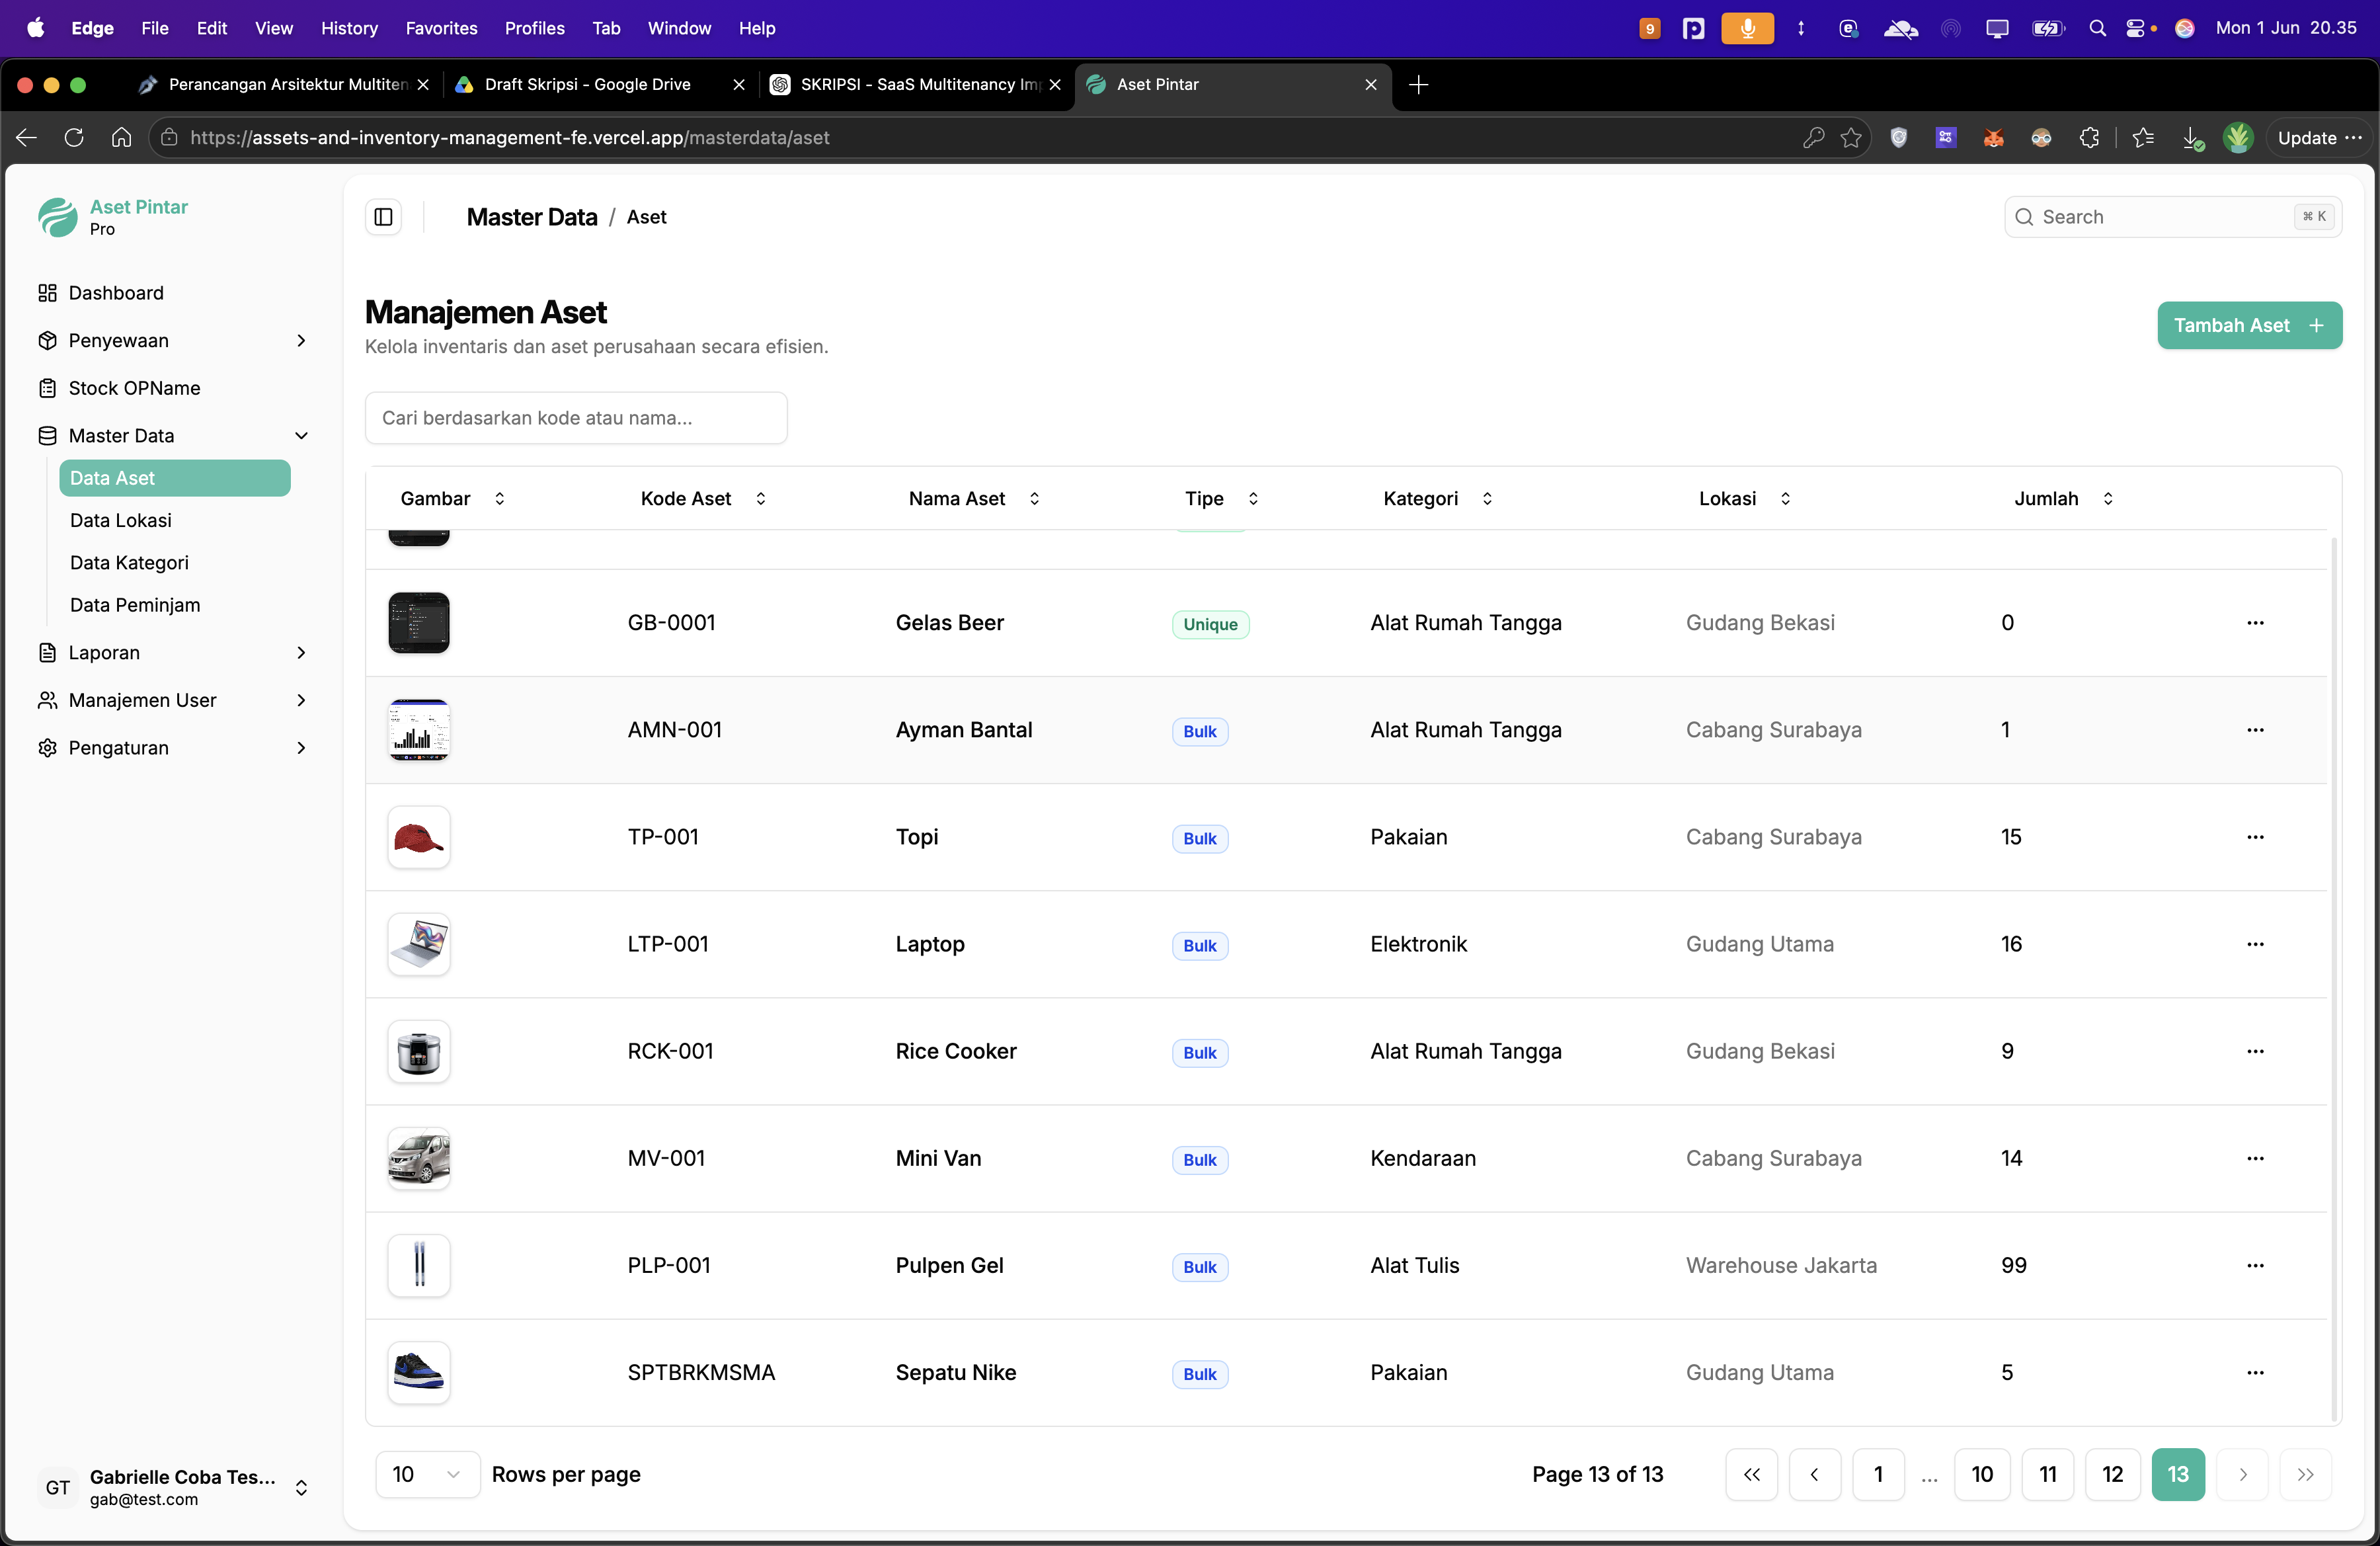
\includegraphics[width=0.9\textwidth]{assets/bab4/test1/web1.png}
  \caption{Data Aset Tenant A pada Aplikasi}
  \label{fig:data_aset_tenant_a}
\end{figure}

Berdasarkan Gambar \ref{fig:data_aset_tenant_a}, pengguna dengan akun \textbf{gab@test.com} hanya dapat melihat data aset yang dimiliki oleh Tenant A. Seluruh data yang ditampilkan pada halaman pengelolaan aset berasal dari \textit{tenant} yang sama dengan akun yang digunakan untuk login. Data milik \textit{tenant} lain tidak ditampilkan pada halaman tersebut meskipun tersimpan pada basis data yang sama.

\begin{figure}[H]
  \centering
  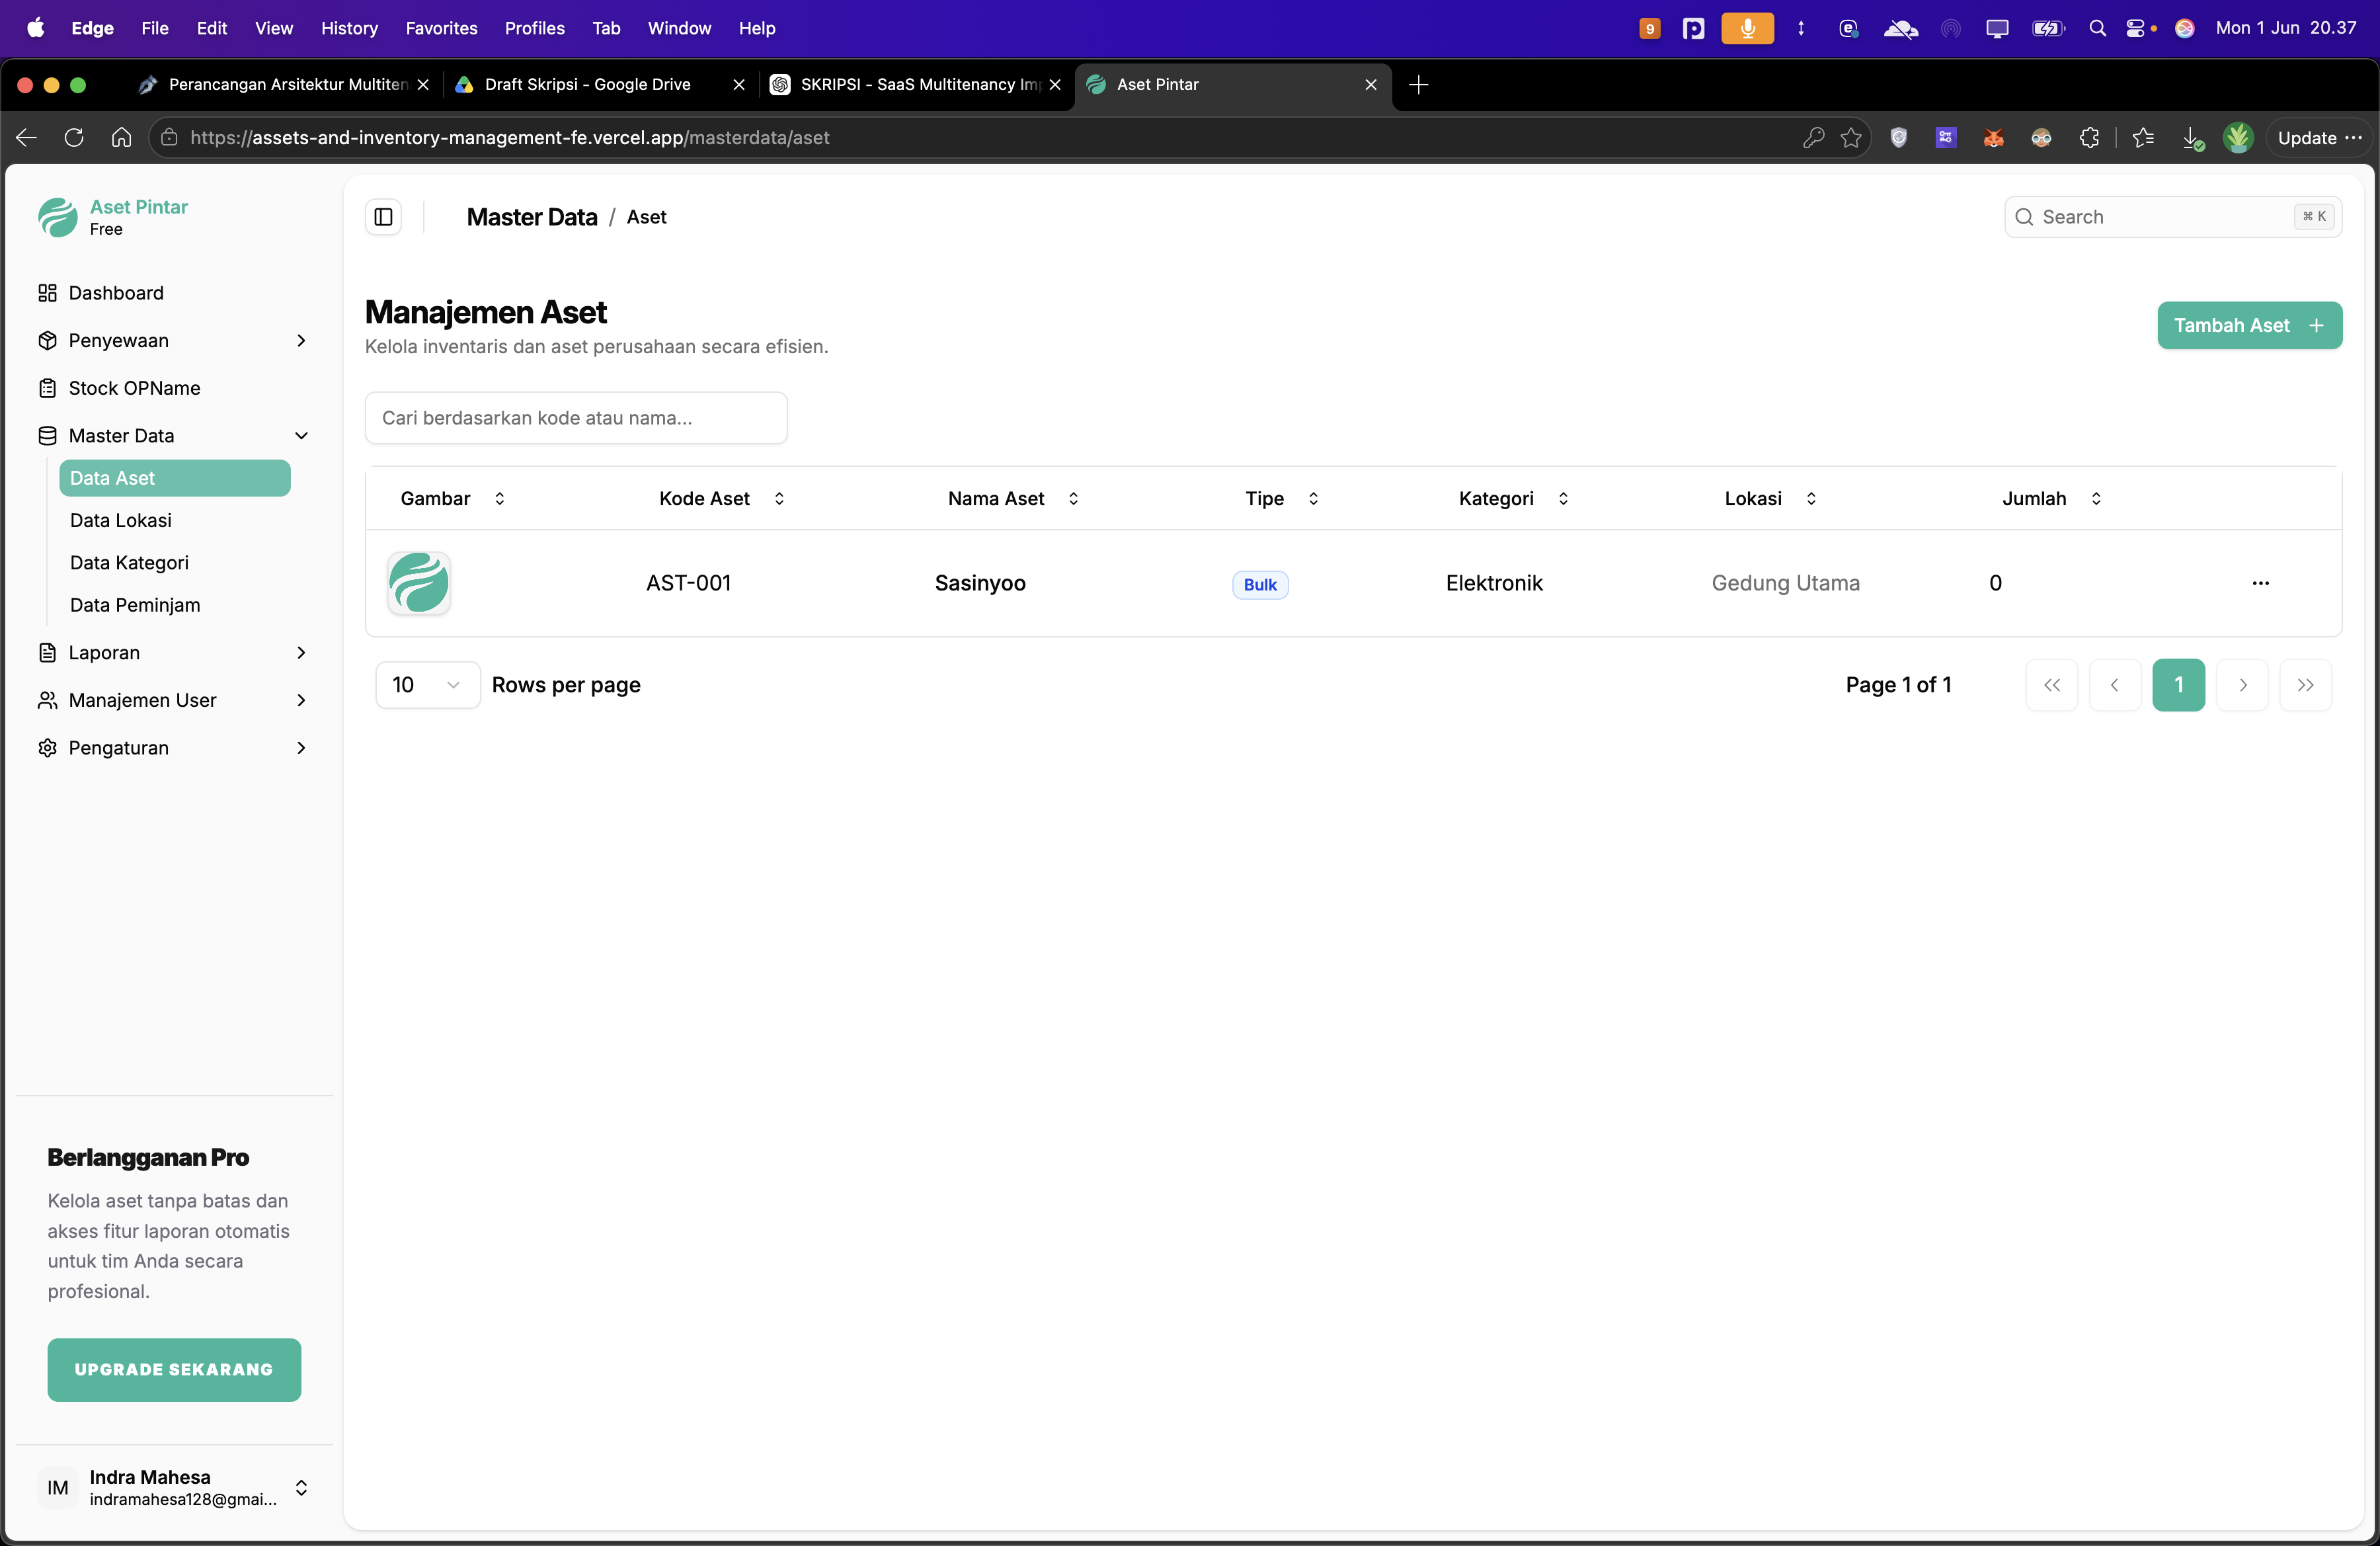
\includegraphics[width=0.9\textwidth]{assets/bab4/test1/web2.png}
  \caption{Data Aset Tenant B pada Aplikasi}
  \label{fig:data_aset_tenant_b}
\end{figure}

Hasil pengujian pada Gambar \ref{fig:data_aset_tenant_b} menunjukkan bahwa pengguna dengan akun \textbf{indramahesa128@gmail.com} hanya dapat mengakses data aset yang dimiliki oleh Tenant B. Data yang ditampilkan berbeda dengan data yang diperoleh oleh Tenant A. Hal tersebut menunjukkan bahwa sistem berhasil menerapkan pemfilteran data berdasarkan identitas \textit{tenant} yang diperoleh pada saat proses autentikasi.

Untuk memastikan bahwa data kedua \textit{tenant} memang tersimpan pada basis data yang sama, dilakukan pemeriksaan langsung pada tabel \textit{assets}. Hasil pemeriksaan ditunjukkan pada Gambar \ref{fig:data_aset_database}.

\begin{figure}[H]
  \centering
  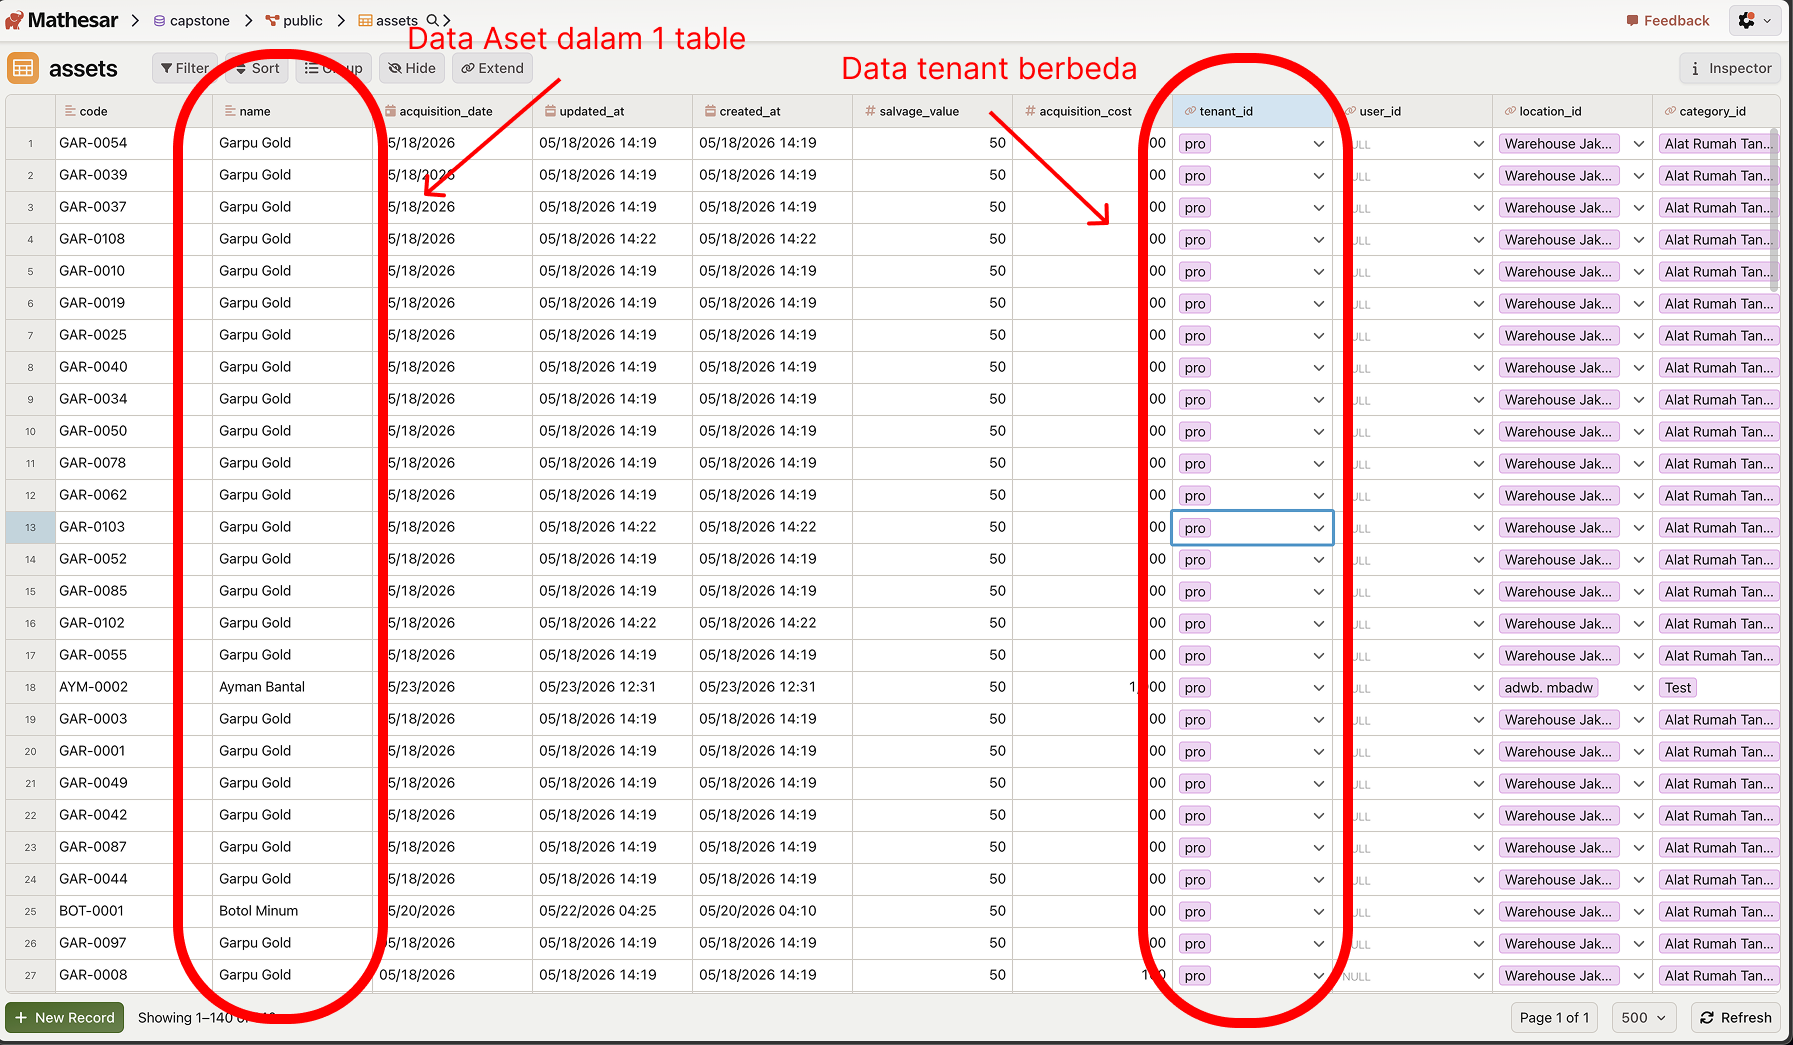
\includegraphics[width=0.9\textwidth]{assets/bab4/test1/db.png}
  \caption{Data Aset Beberapa \textit{Tenant} pada Tabel \textit{Assets}}
  \label{fig:data_aset_database}
\end{figure}

Berdasarkan Gambar \ref{fig:data_aset_database}, data aset dari Tenant A dan Tenant B tersimpan pada tabel \textit{assets} yang sama. Setiap data memiliki atribut \textit{tenant\_id} yang digunakan sebagai identitas kepemilikan data. Atribut tersebut menjadi dasar bagi sistem untuk menentukan data mana yang dapat diakses oleh \textit{tenant} yang sedang aktif. Dengan demikian, meskipun seluruh \textit{tenant} menggunakan tabel yang sama, sistem tetap mampu menjaga pemisahan data antar \textit{tenant}.

Selain melalui antarmuka aplikasi, verifikasi juga dilakukan pada lapisan layanan API. Pengujian ini bertujuan untuk memastikan bahwa mekanisme \textit{tenant isolation} diterapkan secara konsisten pada seluruh lapisan sistem dan tidak hanya pada tampilan aplikasi.

\begin{figure}[H]
  \centering
  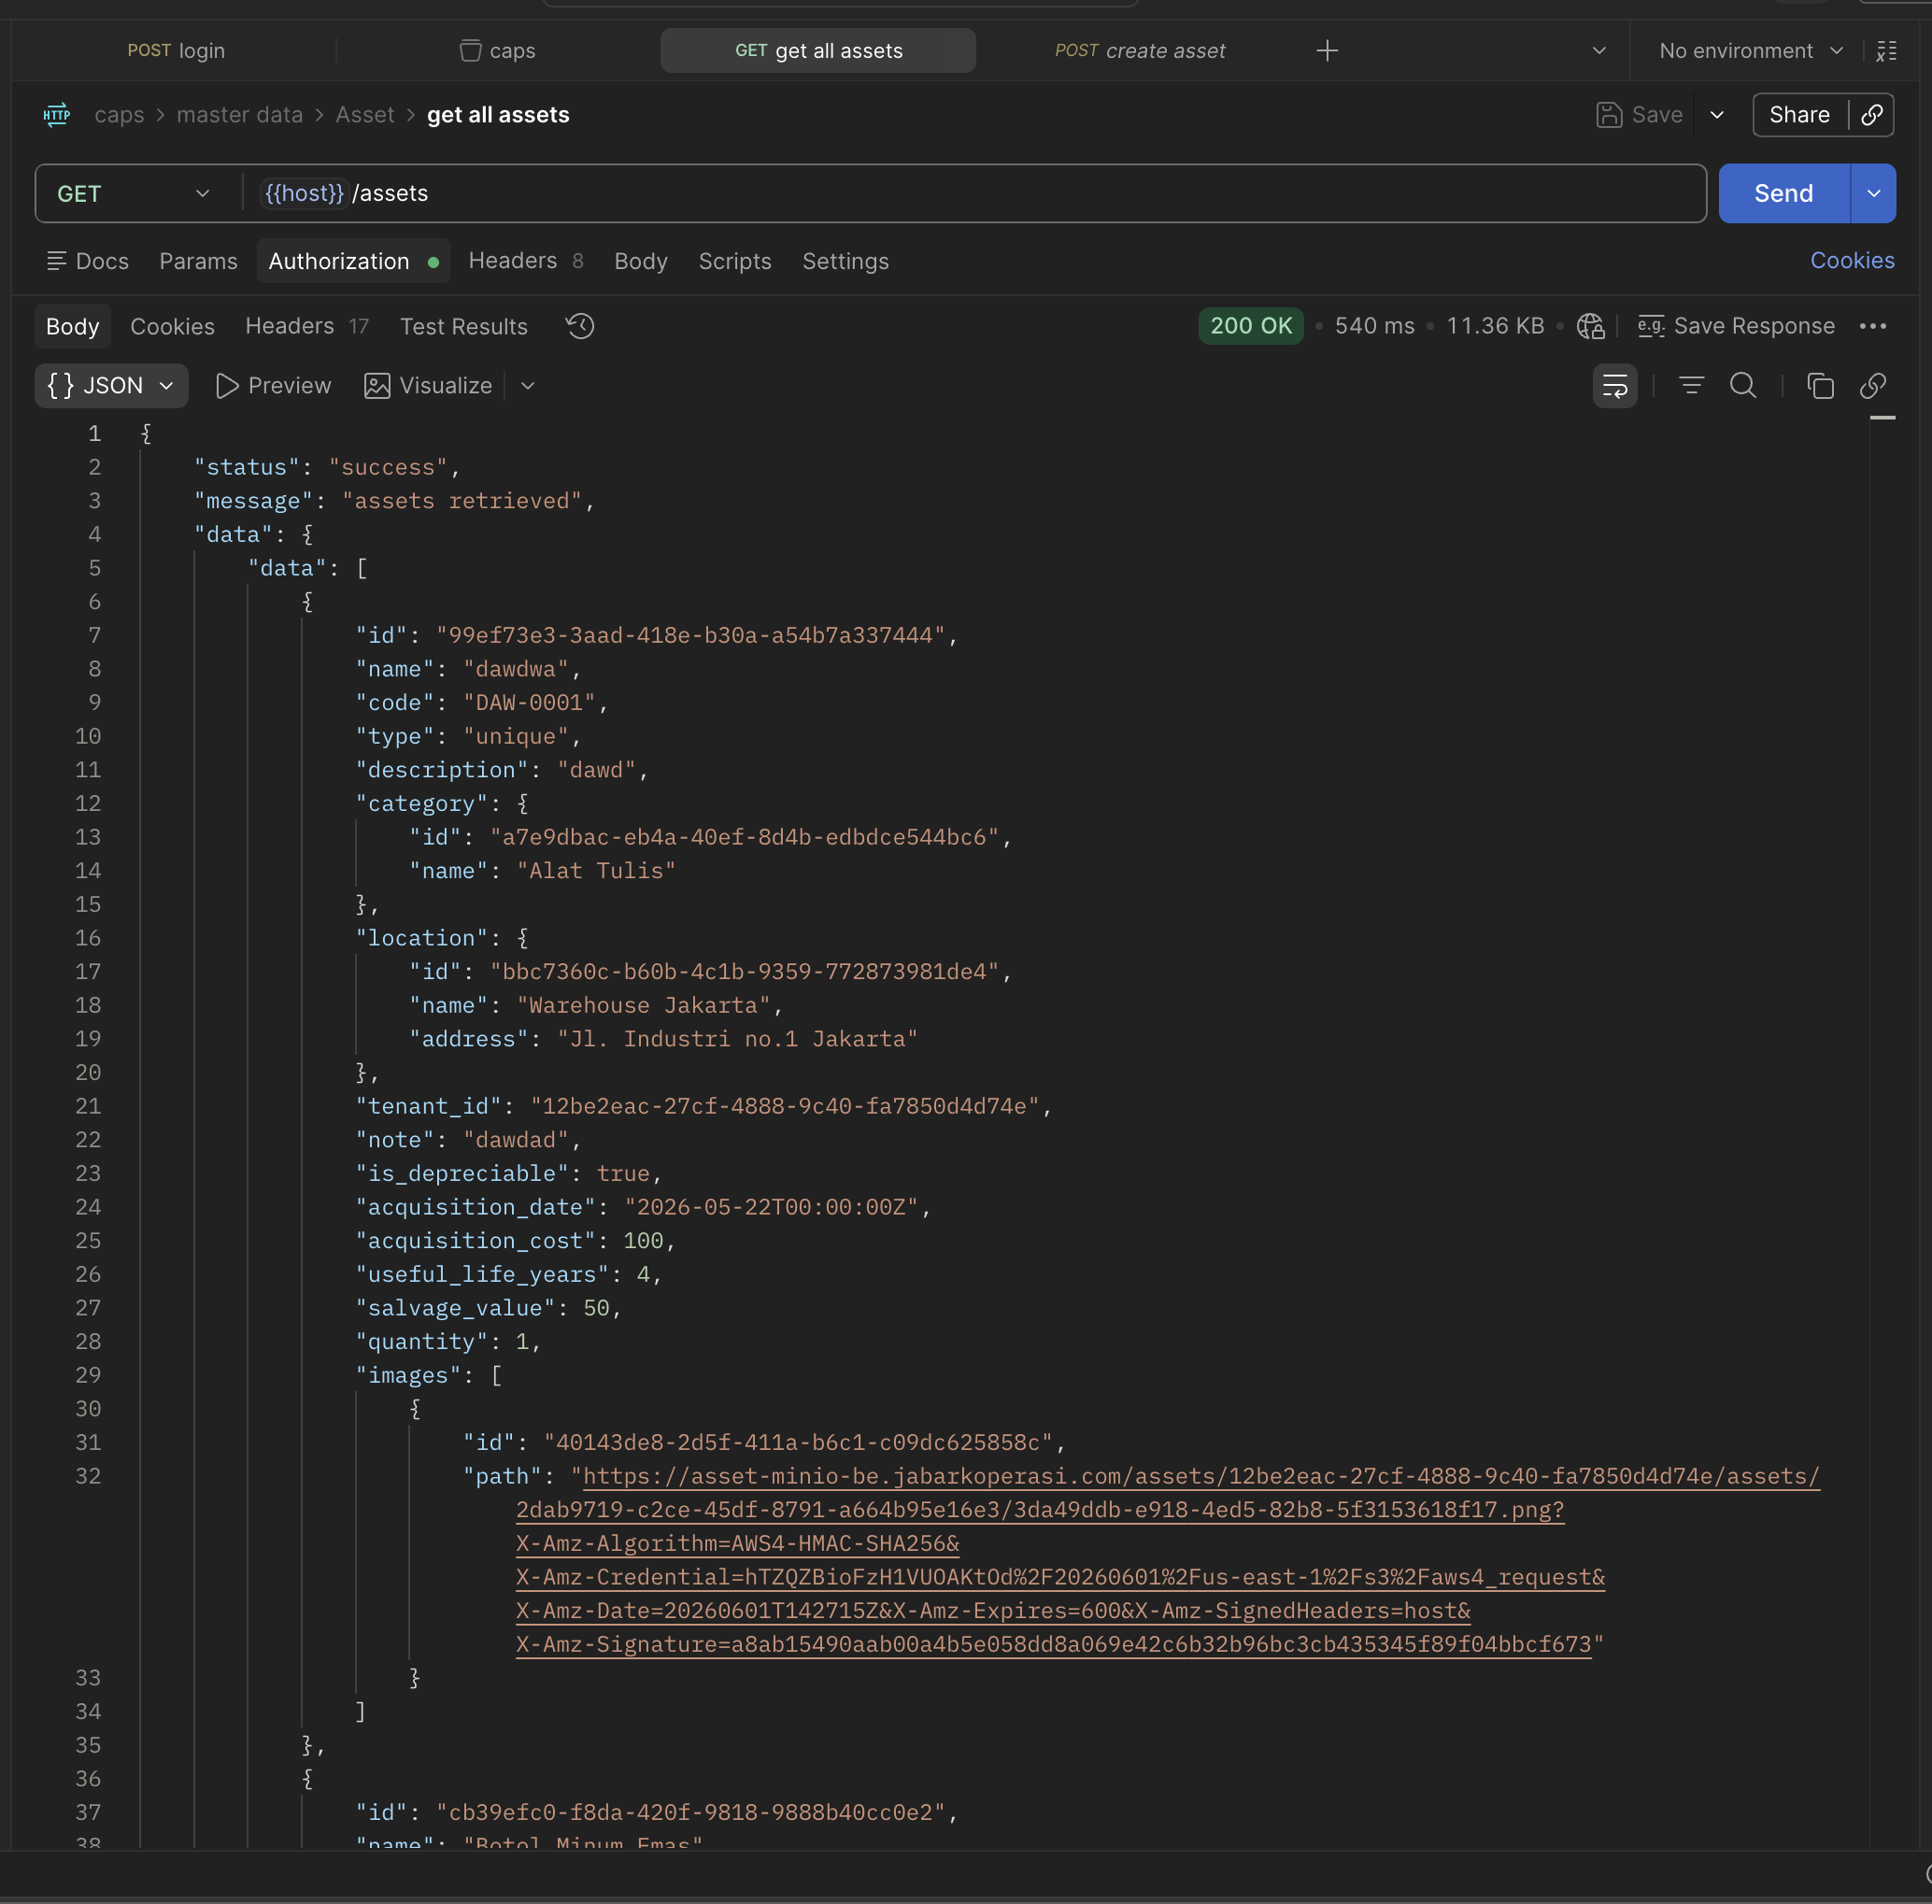
\includegraphics[width=0.9\textwidth]{assets/bab4/test1/api1.png}
  \caption{Respons API Pengambilan Data Aset Tenant A}
  \label{fig:api_tenant_a}
\end{figure}

Berdasarkan Gambar \ref{fig:api_tenant_a}, layanan API hanya mengembalikan data aset yang dimiliki Tenant A. Data yang berasal dari Tenant B tidak terdapat pada respons yang diterima pengguna. Hasil tersebut menunjukkan bahwa identitas \textit{tenant} yang tersimpan pada token autentikasi berhasil digunakan sebagai parameter pembatas akses data.

\begin{figure}[H]
  \centering
  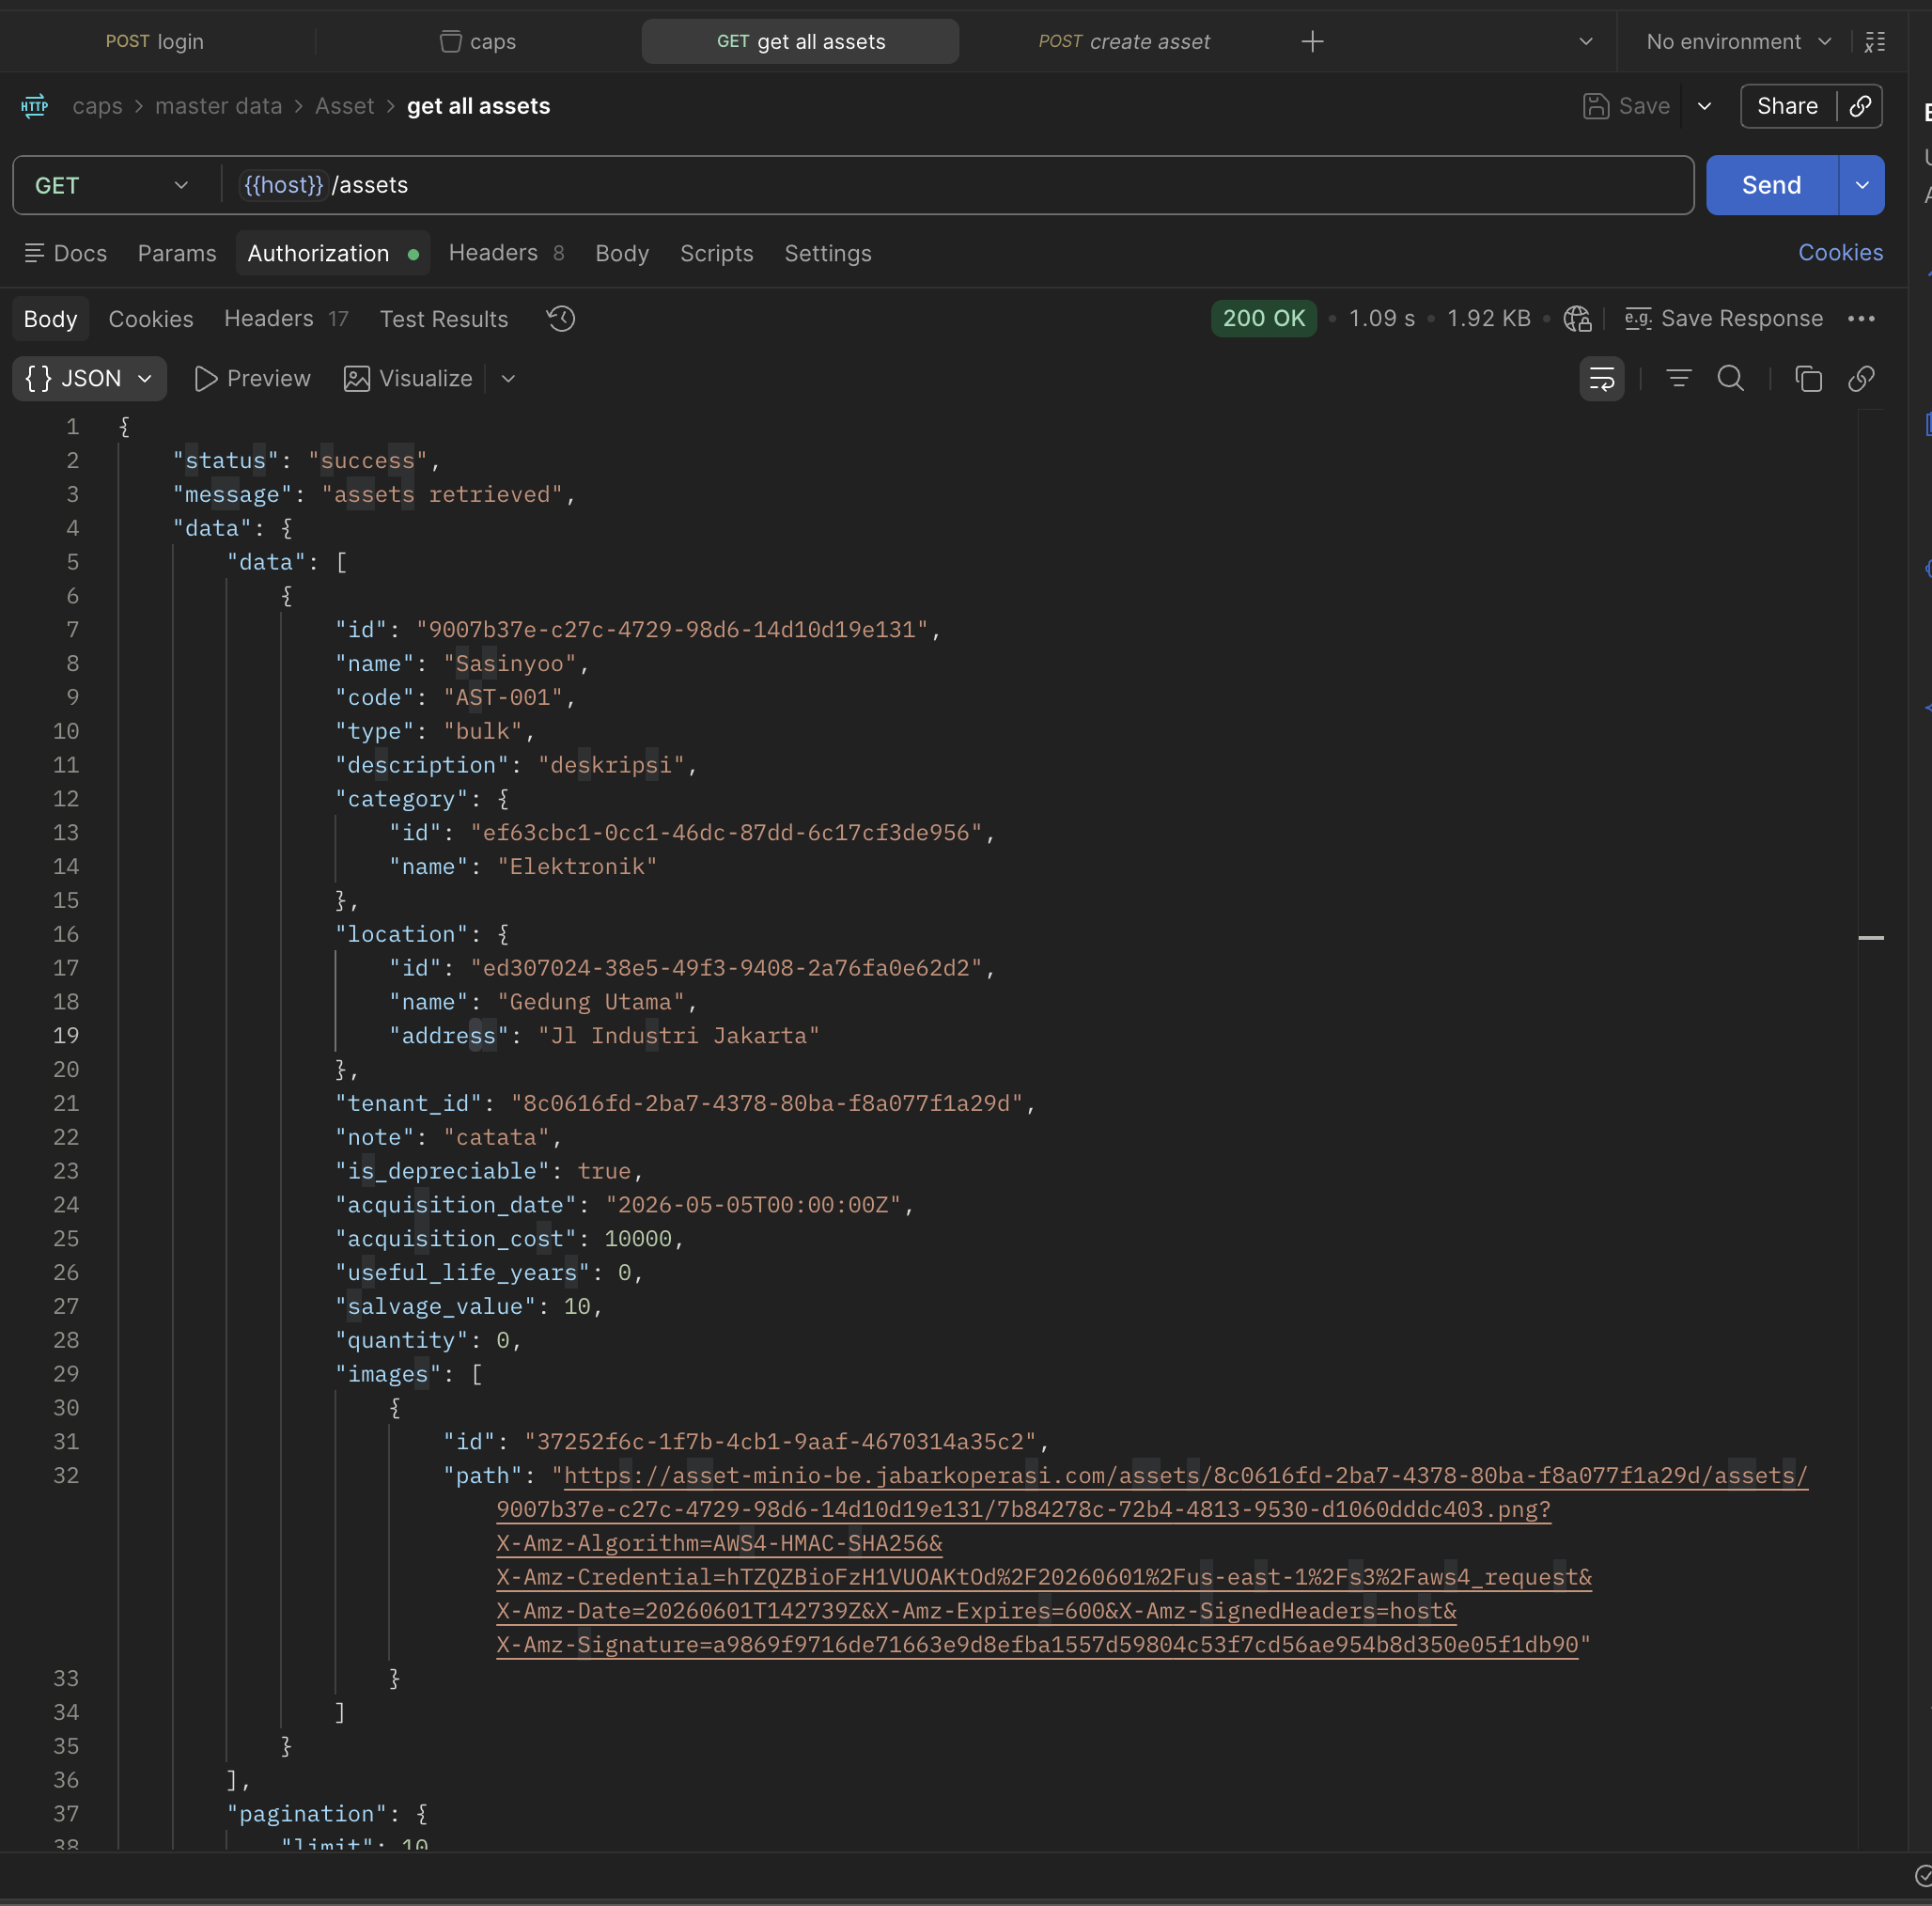
\includegraphics[width=0.9\textwidth]{assets/bab4/test1/api2.png}
  \caption{Respons API Pengambilan Data Aset Tenant B}
  \label{fig:api_tenant_b}
\end{figure}

Hasil yang ditunjukkan pada Gambar \ref{fig:api_tenant_b} memperlihatkan bahwa pengguna Tenant B memperoleh data yang berbeda dengan Tenant A. Sistem hanya mengembalikan data yang memiliki keterkaitan dengan \textit{tenant} yang sedang aktif. Dengan demikian, akses terhadap data \textit{tenant} lain dapat dicegah meskipun permintaan dilakukan melalui \textit{endpoint} API yang sama.

Untuk mempermudah evaluasi hasil pengujian, ringkasan hasil pengujian \textit{tenant isolation} disajikan pada Tabel \ref{tab:hasil_pengujian_tenant_isolation}.

\begin{table}[H]
  \centering
  \caption{Hasil Pengujian \textit{Tenant Isolation}}
  \label{tab:hasil_pengujian_tenant_isolation}
  \footnotesize
  \begin{tabular}{|c|p{5cm}|p{4cm}|p{2.5cm}|}
    \hline
    \rowcolor[HTML]{EFEFEF}
    \textbf{No} & \textbf{Skenario Pengujian} & \textbf{Hasil yang Diharapkan} & \textbf{Hasil Pengujian} \\
    \hline
    1 & Tenant A mengakses data aset Tenant A & Data berhasil ditampilkan & Berhasil \\
    \hline
    2 & Tenant B mengakses data aset Tenant B & Data berhasil ditampilkan & Berhasil \\
    \hline
    3 & Tenant A mencoba mengakses data Tenant B & Data tidak ditampilkan & Berhasil \\
    \hline
    4 & Tenant B mencoba mengakses data Tenant A & Data tidak ditampilkan & Berhasil \\
    \hline
    5 & \textit{Tenant} melakukan perubahan data aset & Perubahan hanya berlaku pada data \textit{tenant} terkait & Berhasil \\
    \hline
  \end{tabular}
\end{table}

Berdasarkan hasil pengujian pada Tabel \ref{tab:hasil_pengujian_tenant_isolation}, seluruh skenario pengujian berhasil dijalankan sesuai dengan hasil yang diharapkan. Pengguna hanya dapat mengakses data yang berada dalam ruang lingkup \textit{tenant} yang sesuai, baik melalui antarmuka aplikasi maupun layanan API. Selain itu, pemeriksaan pada basis data menunjukkan bahwa data dari beberapa \textit{tenant} dapat disimpan pada tabel yang sama tanpa menyebabkan pencampuran data.

Hasil tersebut menunjukkan bahwa mekanisme \textit{tenant isolation} yang dirancang pada penelitian ini berhasil diterapkan pada lapisan aplikasi, layanan API, dan basis data. Dengan demikian, pendekatan \textit{shared database} dan \textit{shared schema} yang digunakan tetap mampu menjaga pemisahan data antar \textit{tenant} sesuai dengan tujuan penelitian yang telah ditetapkan.

\subsection{Hasil Pengujian Tenant Provisioning}

Pengujian \textit{tenant provisioning} dilakukan untuk memverifikasi bahwa proses registrasi \textit{tenant} baru dapat berjalan secara otomatis sesuai dengan rancangan yang telah dijelaskan pada Bab 3. Pengujian ini bertujuan untuk memastikan bahwa sistem mampu membuat \textit{tenant} baru beserta seluruh konfigurasi awal yang diperlukan, sehingga \textit{tenant} dapat langsung menggunakan sistem setelah proses registrasi selesai.

Pada pengujian ini, dilakukan registrasi \textit{tenant} baru menggunakan data organisasi dan akun administrator yang belum pernah terdaftar pada sistem. Setelah proses registrasi berhasil dilakukan, verifikasi dilakukan terhadap data \textit{tenant}, \textit{role} administrator, \textit{permission}, serta akun administrator yang terbentuk secara otomatis pada basis data.

\begin{figure}[H]
  \centering
  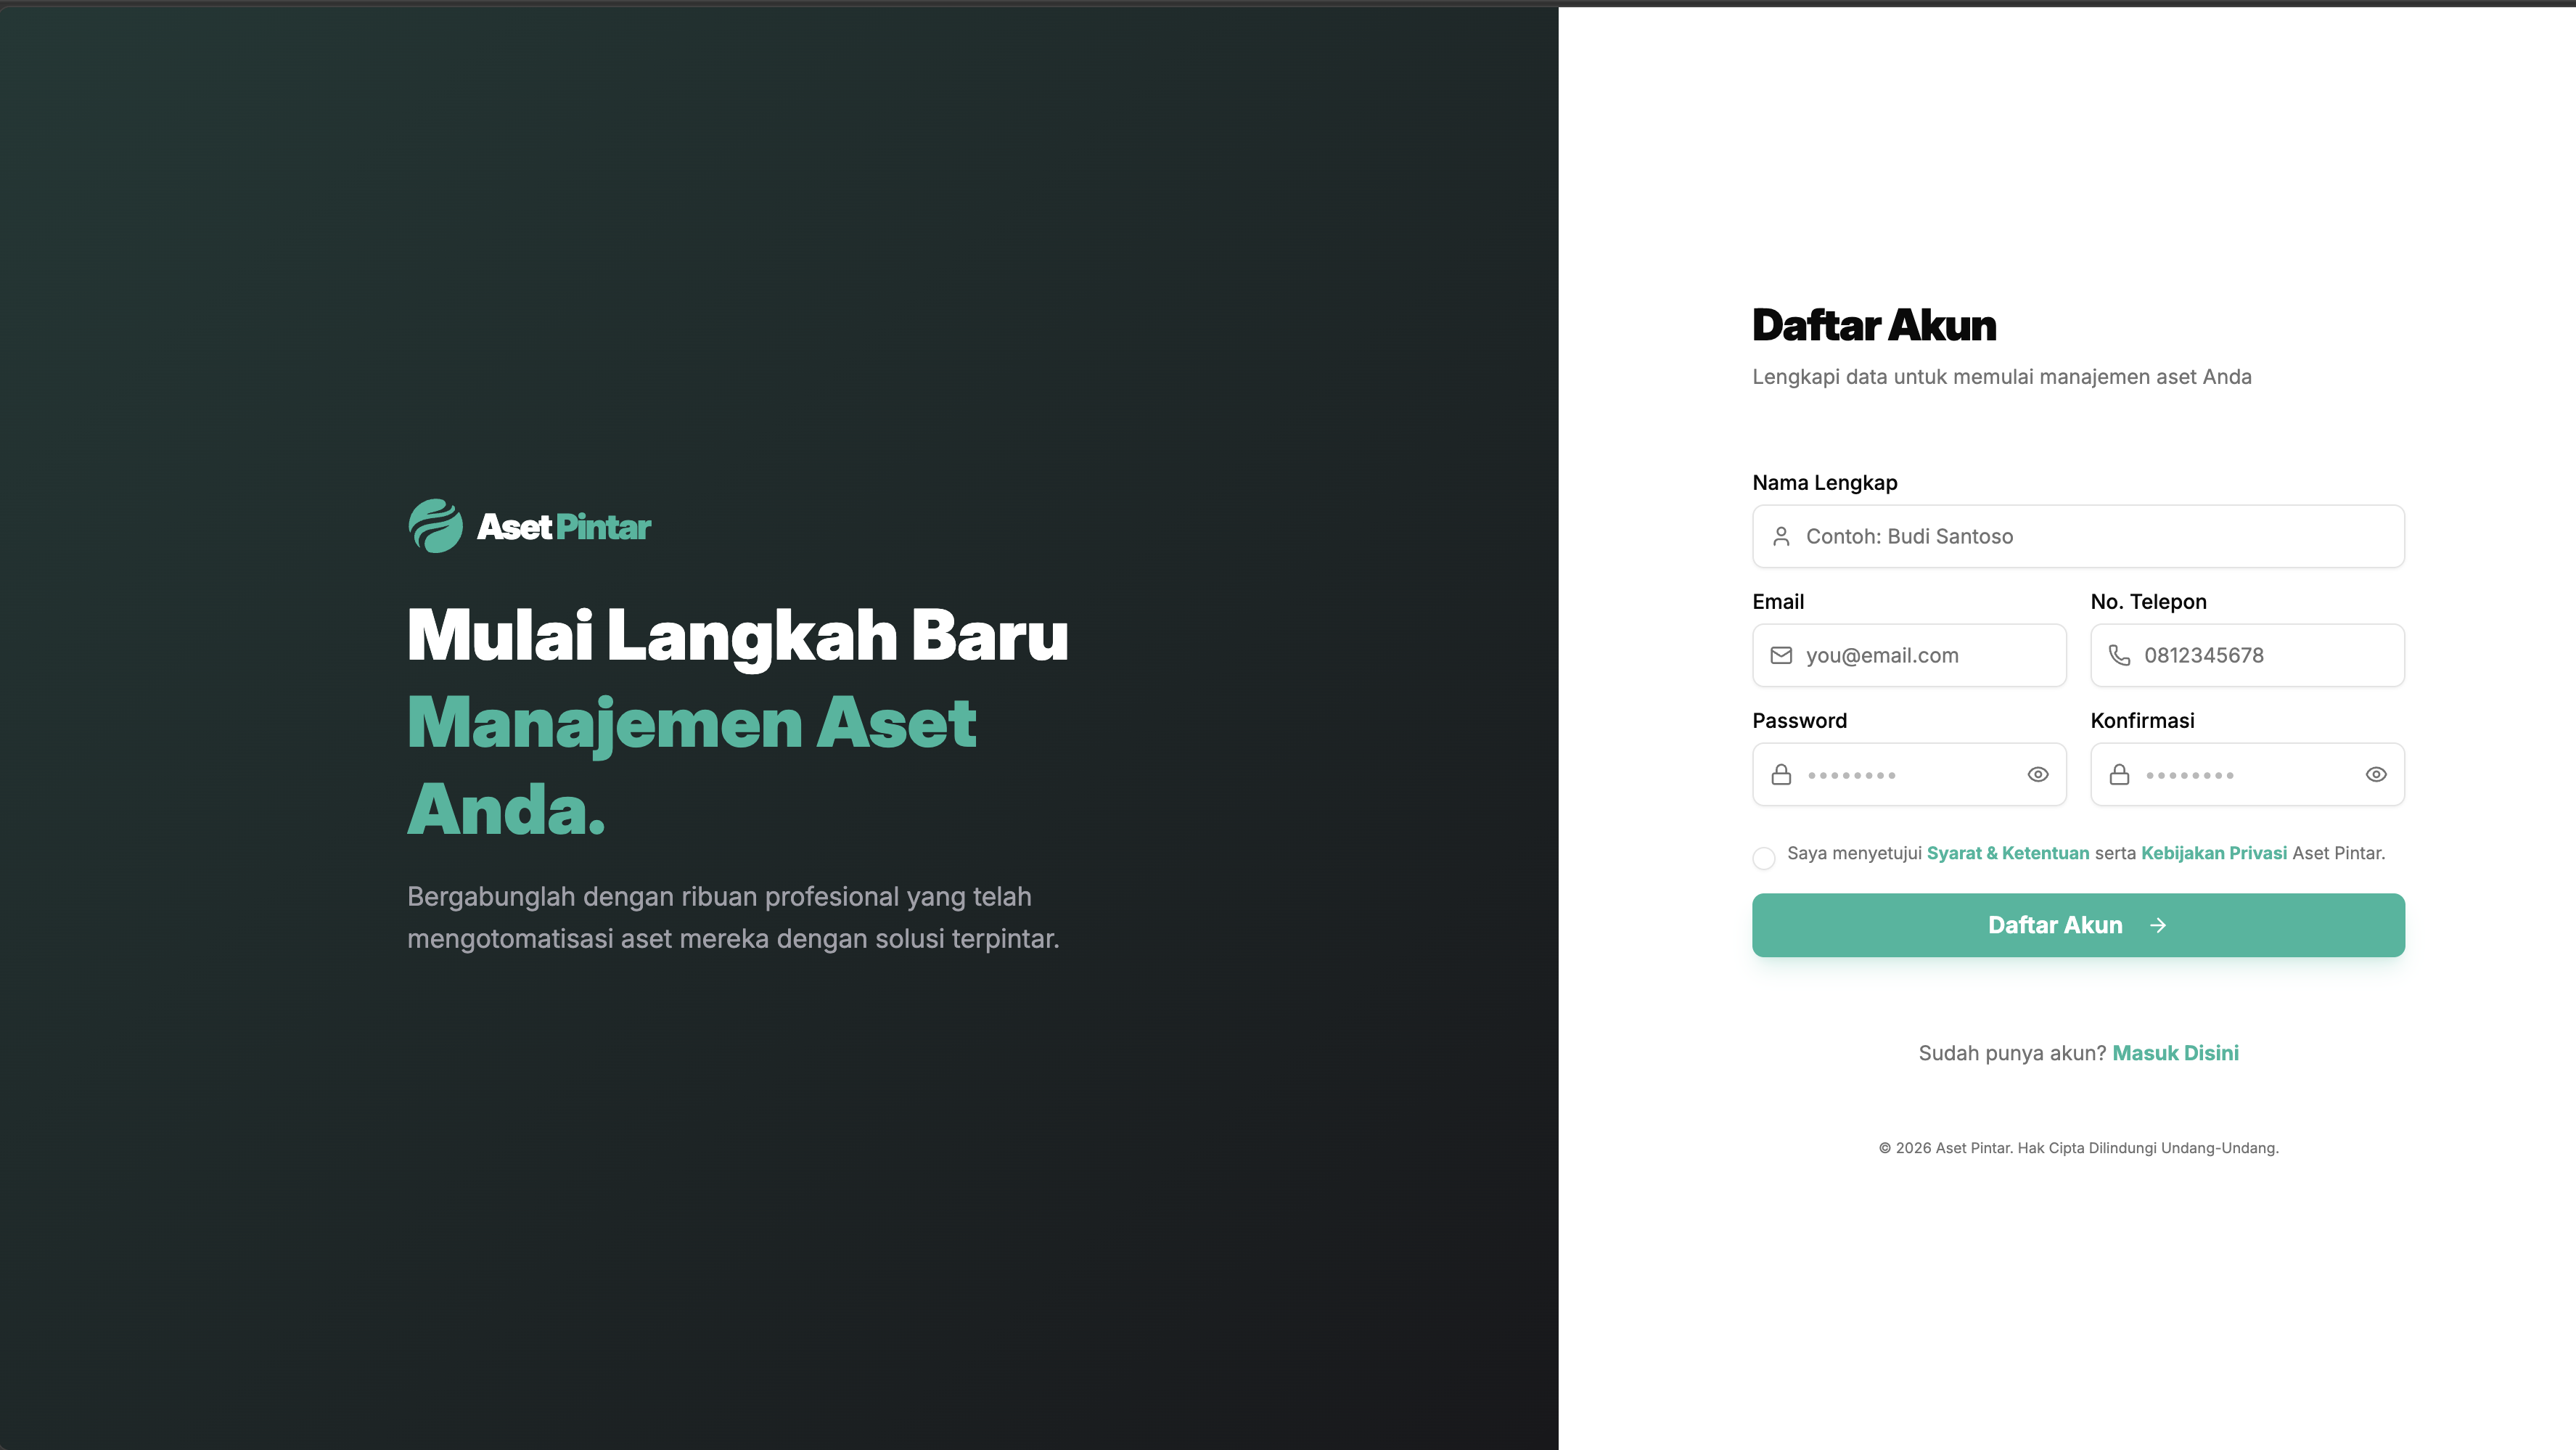
\includegraphics[width=0.9\textwidth]{assets/bab4/test2/signup.png}
  \caption{Form Registrasi \textit{Tenant} Baru}
  \label{fig:form_registrasi_tenant}
\end{figure}

Berdasarkan Gambar \ref{fig:form_registrasi_tenant}, pengguna mengisi informasi yang diperlukan untuk proses registrasi \textit{tenant}. Informasi tersebut mencakup data \textit{tenant} dan akun administrator yang akan digunakan untuk mengakses sistem setelah proses registrasi berhasil dilakukan.

Setelah proses registrasi berhasil dijalankan, sistem secara otomatis membuat data \textit{tenant} baru pada tabel \textit{tenants}. Hasil pembentukan data \textit{tenant} ditunjukkan pada Gambar \ref{fig:data_tenant_baru}.

\begin{figure}[H]
  \centering
  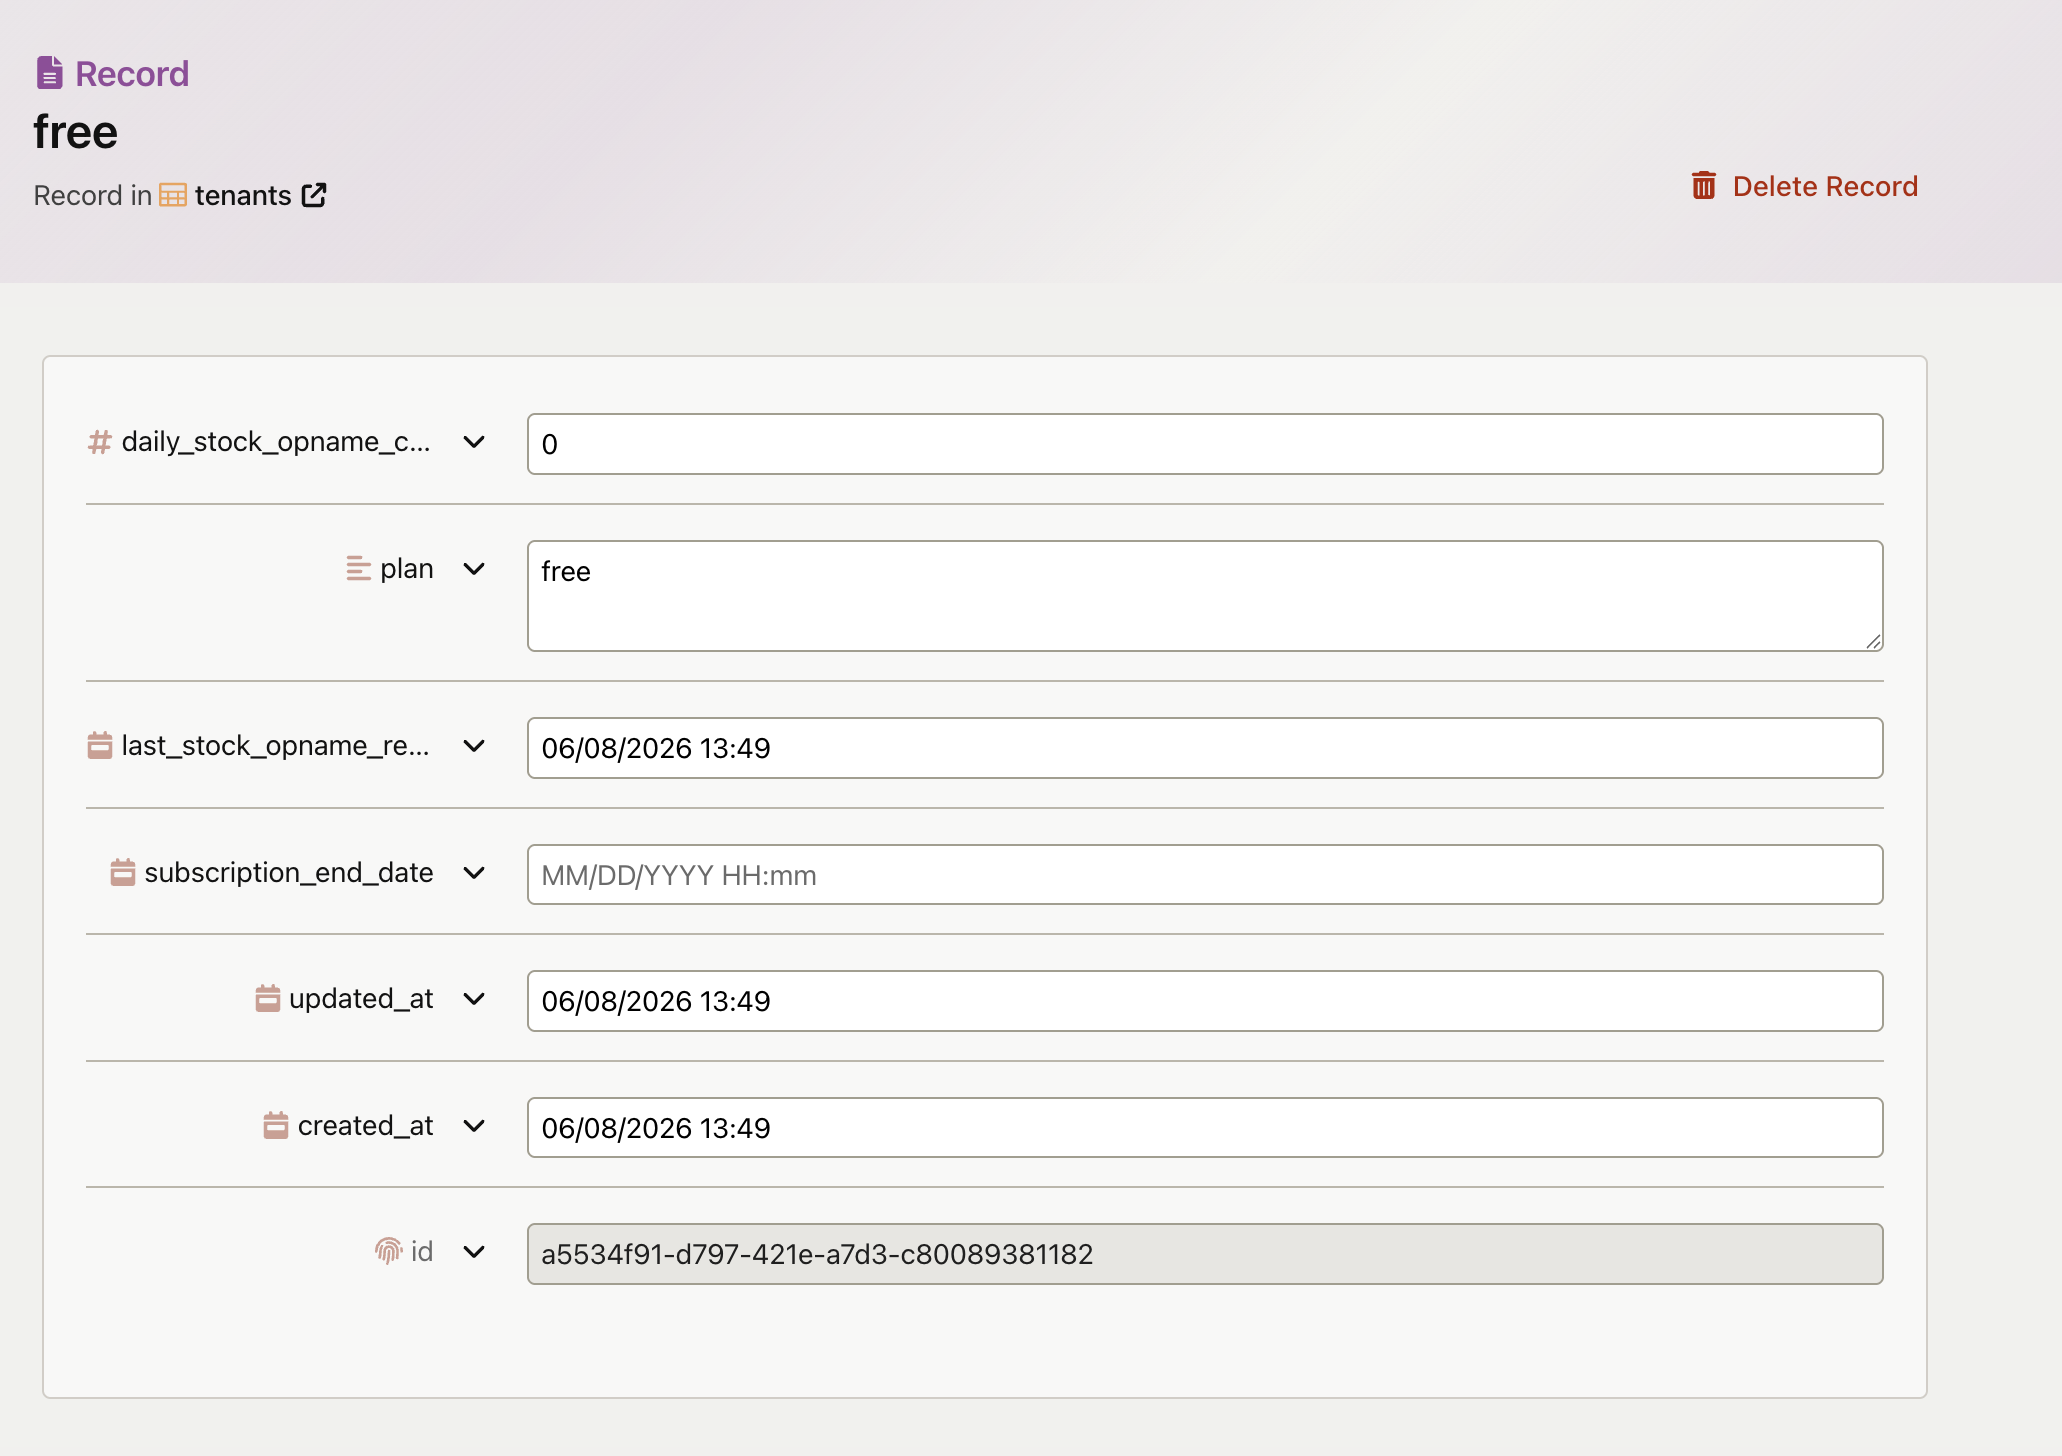
\includegraphics[width=0.9\textwidth]{assets/bab4/test2/table-tenant.png}
  \caption{Data \textit{Tenant} yang Berhasil Dibuat}
  \label{fig:data_tenant_baru}
\end{figure}

Berdasarkan Gambar \ref{fig:data_tenant_baru}, sistem berhasil membuat data \textit{tenant} baru dan menghasilkan identitas \textit{tenant} (\textit{tenant\_id}) yang digunakan sebagai referensi pada proses berikutnya. Identitas tersebut menjadi dasar untuk menghubungkan seluruh data yang dimiliki oleh \textit{tenant}.

Tahap berikutnya adalah pembuatan \textit{role} administrator yang akan digunakan untuk mengelola \textit{tenant} yang baru terdaftar. Hasil pembentukan \textit{role} administrator ditunjukkan pada Gambar \ref{fig:data_role_administrator}.

\begin{figure}[H]
  \centering
  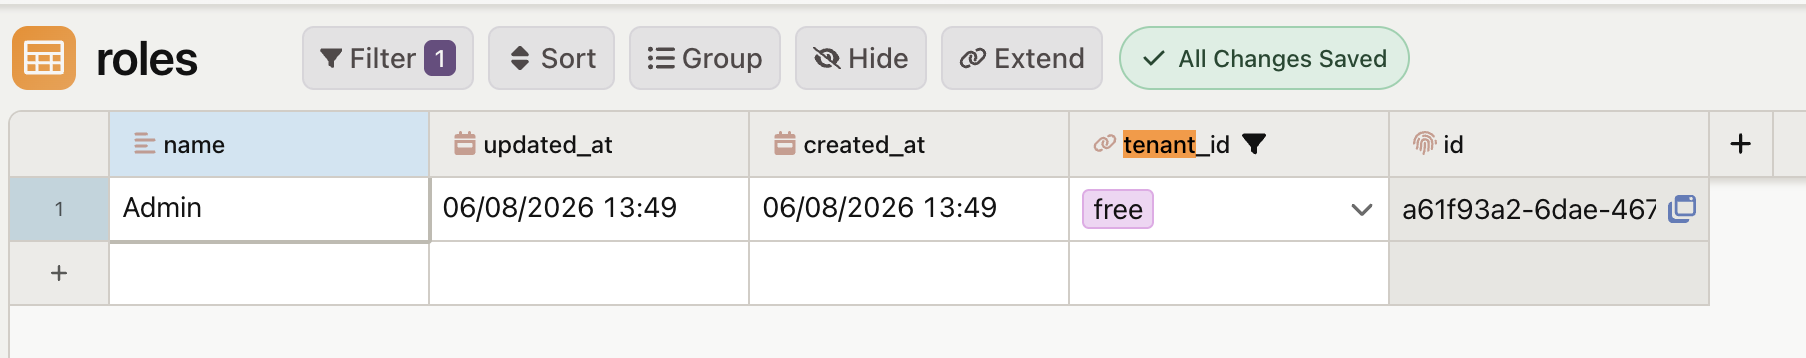
\includegraphics[width=0.9\textwidth]{assets/bab4/test2/table-role.png}
  \caption{Data \textit{Role} Administrator \textit{Tenant}}
  \label{fig:data_role_administrator}
\end{figure}

Hasil pada Gambar \ref{fig:data_role_administrator} menunjukkan bahwa sistem berhasil membuat \textit{role} administrator yang terhubung dengan \textit{tenant} yang baru dibuat. \textit{Role} tersebut digunakan sebagai dasar dalam pengelolaan hak akses pengguna pada \textit{tenant} terkait.

Setelah \textit{role} administrator berhasil dibuat, sistem secara otomatis memberikan hak akses melalui relasi antara \textit{role} dan \textit{permission}. Hasil proses tersebut ditunjukkan pada Gambar \ref{fig:relasi_role_permission}.

\begin{figure}[H]
  \centering
  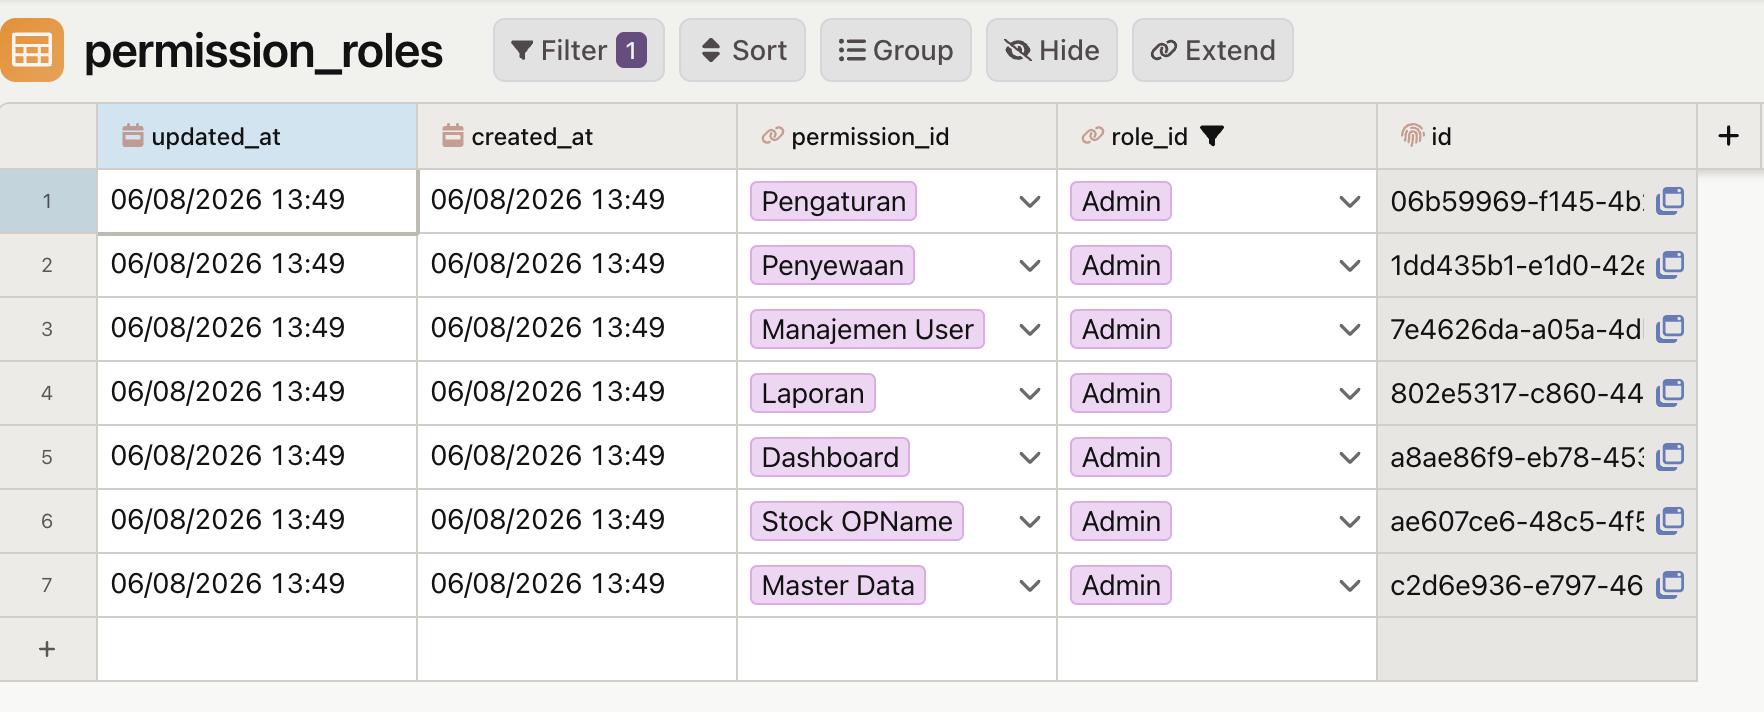
\includegraphics[width=0.9\textwidth]{assets/bab4/test2/table-permission.png}
  \caption{Relasi \textit{Role} Administrator dengan \textit{Permission}}
  \label{fig:relasi_role_permission}
\end{figure}

Berdasarkan Gambar \ref{fig:relasi_role_permission}, \textit{role} administrator berhasil dikaitkan dengan seluruh \textit{permission} yang diperlukan untuk mengakses fitur sistem. Dengan konfigurasi tersebut, administrator \textit{tenant} dapat melakukan pengelolaan data tanpa memerlukan konfigurasi tambahan setelah proses registrasi selesai.

Selanjutnya, sistem membuat akun administrator berdasarkan informasi yang diberikan saat registrasi. Hasil pembentukan akun administrator ditunjukkan pada Gambar \ref{fig:data_akun_administrator}.

\begin{figure}[H]
  \centering
  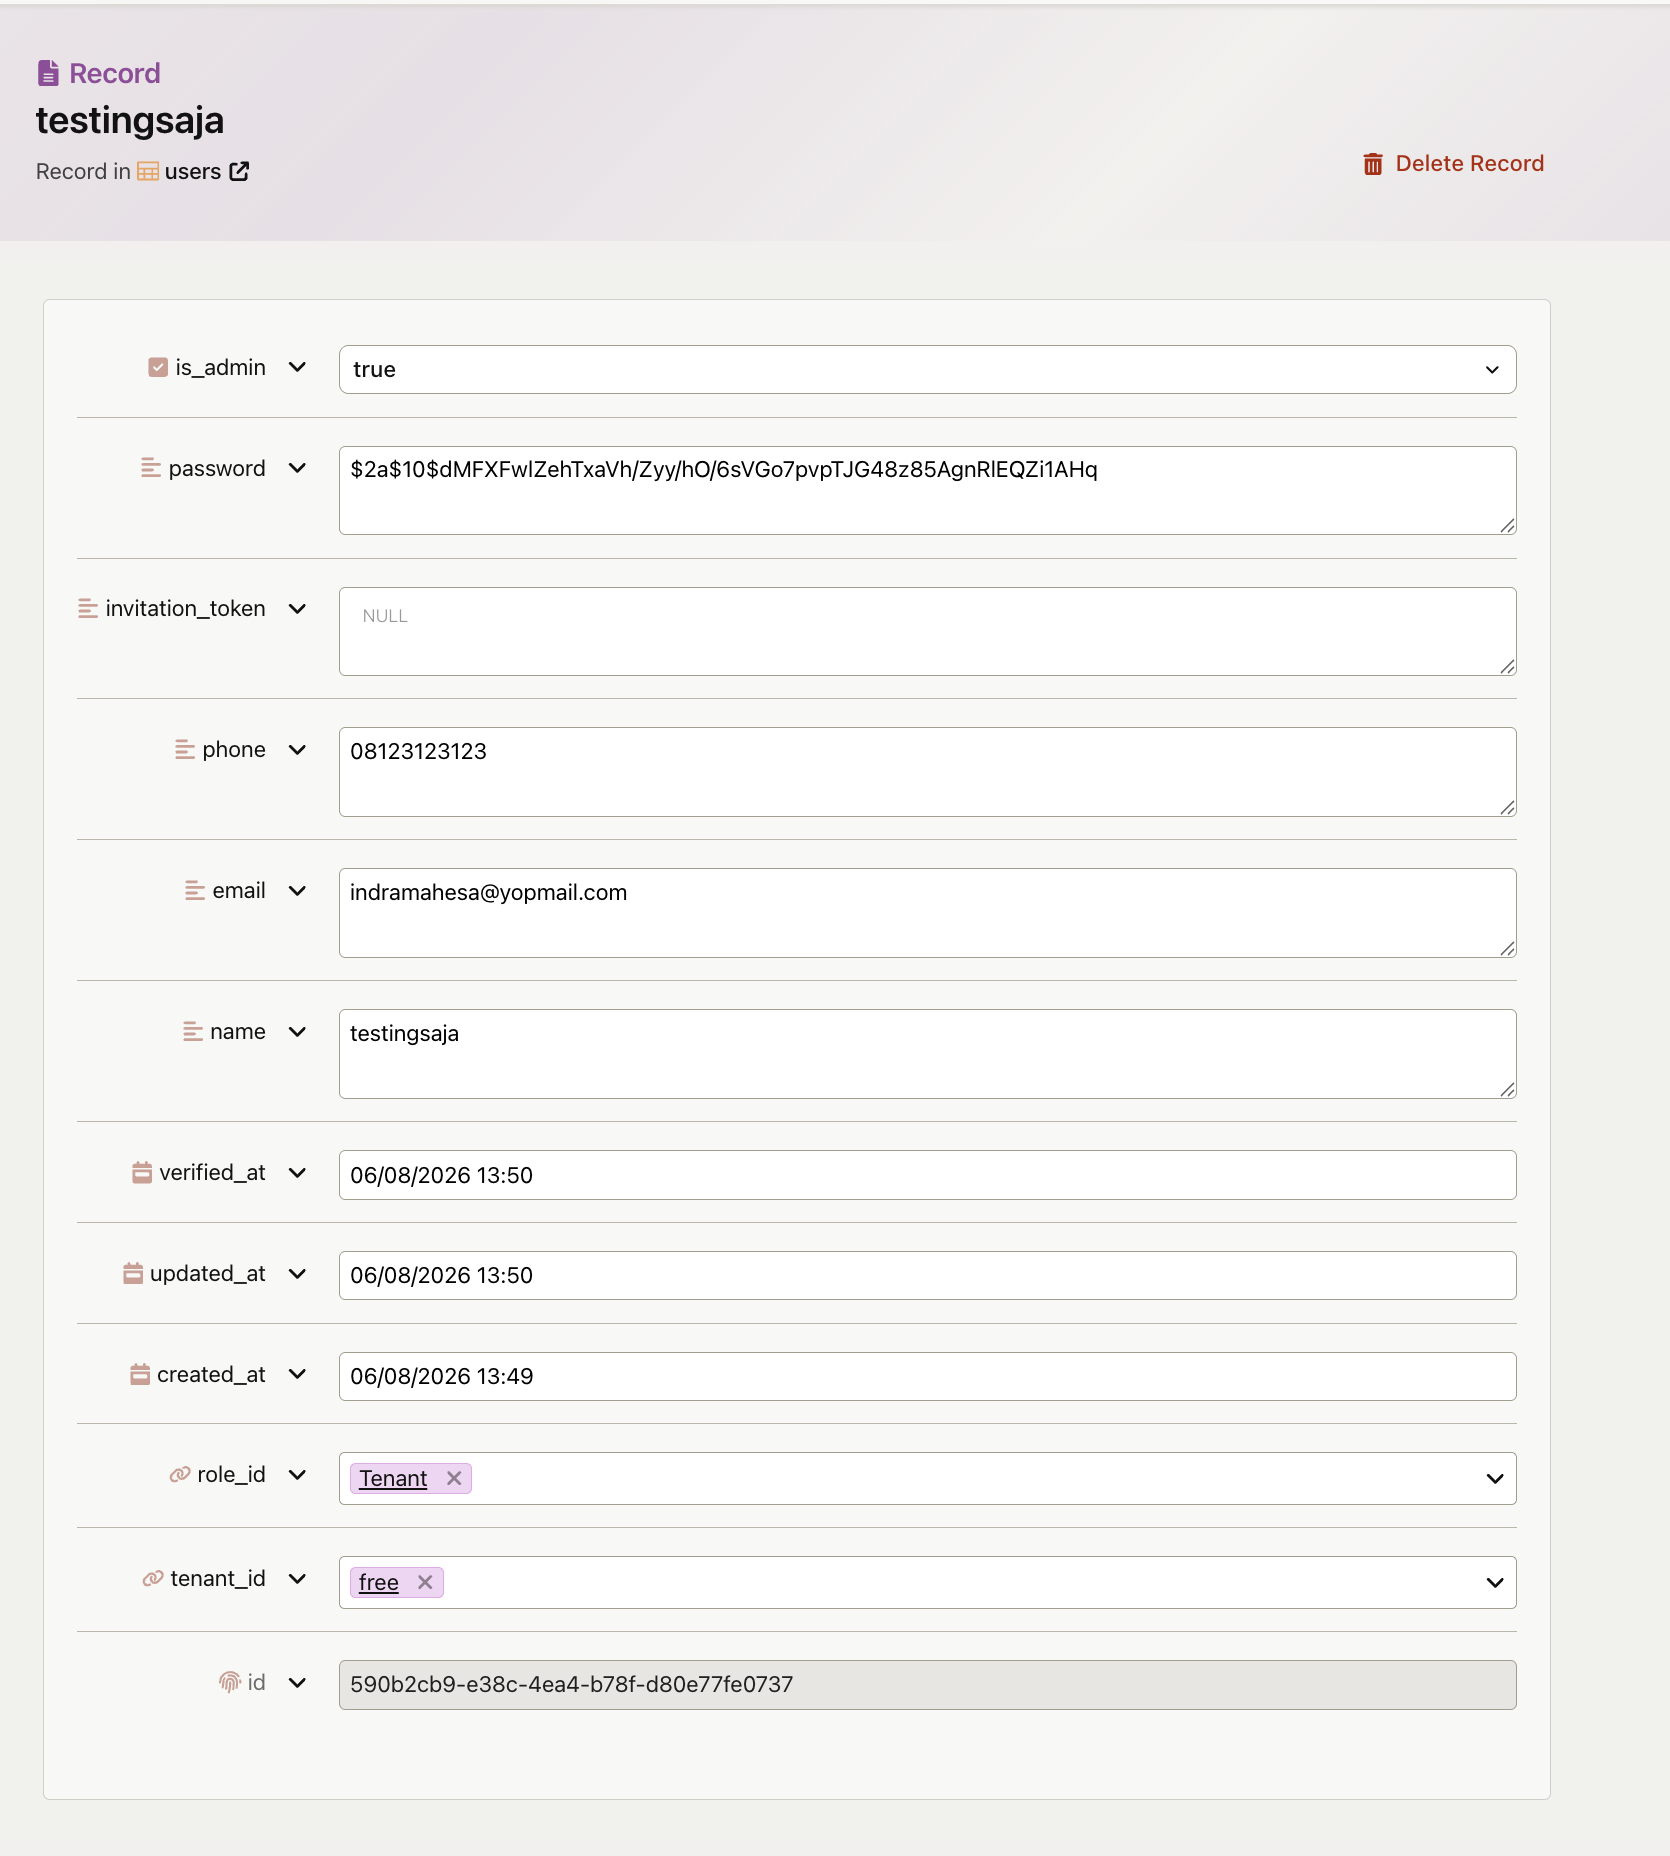
\includegraphics[width=0.9\textwidth]{assets/bab4/test2/table-user.png}
  \caption{Data Akun Administrator \textit{Tenant}}
  \label{fig:data_akun_administrator}
\end{figure}

Berdasarkan Gambar \ref{fig:data_akun_administrator}, akun administrator berhasil dibuat dan dikaitkan dengan \textit{tenant} yang sesuai. Selain itu, akun tersebut juga telah terhubung dengan \textit{role} administrator yang sebelumnya dibuat oleh sistem.

Untuk mempermudah evaluasi hasil pengujian, ringkasan hasil pengujian \textit{tenant provisioning} disajikan pada Tabel \ref{tab:hasil_pengujian_tenant_provisioning}.

\begin{table}[H]
  \centering
  \caption{Hasil Pengujian \textit{Tenant Provisioning}}
  \label{tab:hasil_pengujian_tenant_provisioning}
  \footnotesize
  \begin{tabular}{|l|>{\raggedright\arraybackslash}p{4.5cm}|>{\raggedright\arraybackslash}p{4.5cm}|>{\raggedright\arraybackslash}p{2.5cm}|}
    \hline
    \rowcolor[HTML]{EFEFEF}
    \textbf{No} & \textbf{Skenario Pengujian} & \textbf{Hasil yang Diharapkan} & \textbf{Hasil Pengujian} \\
    \hline
    1 & Registrasi \textit{tenant} baru & Data \textit{tenant} berhasil dibuat & Berhasil \\
    \hline
    2 & Pembuatan \textit{role} administrator & \textit{Role} administrator berhasil dibuat & Berhasil \\
    \hline
    3 & Pemberian \textit{permission} & \textit{Permission} berhasil dikaitkan dengan \textit{role} administrator & Berhasil \\
    \hline
    4 & Pembuatan akun administrator & Akun administrator berhasil dibuat & Berhasil \\
    \hline
    5 & Relasi pengguna dan \textit{role} & Pengguna berhasil dikaitkan dengan \textit{role} administrator & Berhasil \\
    \hline
    6 & Login menggunakan akun administrator & Pengguna berhasil masuk ke sistem & Berhasil \\
    \hline
  \end{tabular}
\end{table}

Berdasarkan hasil pengujian pada Tabel \ref{tab:hasil_pengujian_tenant_provisioning}, seluruh tahapan \textit{tenant provisioning} berhasil dijalankan sesuai dengan hasil yang diharapkan. Sistem mampu membuat \textit{tenant} baru beserta \textit{role} administrator, \textit{permission}, dan akun administrator secara otomatis tanpa memerlukan konfigurasi manual tambahan.

Hasil tersebut menunjukkan bahwa mekanisme \textit{tenant provisioning} yang diterapkan pada penelitian ini mampu mendukung proses \textit{onboarding} \textit{tenant} secara cepat dan konsisten.

\subsection{Hasil Pengujian Shared Database dan Shared Schema}

Pengujian \textit{shared database} dan \textit{shared schema} dilakukan untuk memverifikasi bahwa beberapa \textit{tenant} dapat menggunakan basis data dan struktur tabel yang sama tanpa menyebabkan pencampuran data antar \textit{tenant}. Pengujian ini penting karena pendekatan yang digunakan pada penelitian ini menempatkan seluruh \textit{tenant} pada satu basis data dan satu struktur tabel yang sama. Oleh karena itu, diperlukan verifikasi untuk memastikan bahwa setiap data tetap dapat diidentifikasi berdasarkan \textit{tenant} yang memilikinya.

Pengujian dilakukan dengan menggunakan beberapa \textit{tenant} yang telah terdaftar pada sistem. Setiap \textit{tenant} melakukan aktivitas pengelolaan data sehingga menghasilkan data operasional yang tersimpan pada basis data. Selanjutnya dilakukan pemeriksaan langsung pada tabel-tabel yang digunakan oleh sistem untuk memastikan bahwa data dari beberapa \textit{tenant} dapat disimpan secara bersamaan.

\begin{figure}[H]
  \centering
  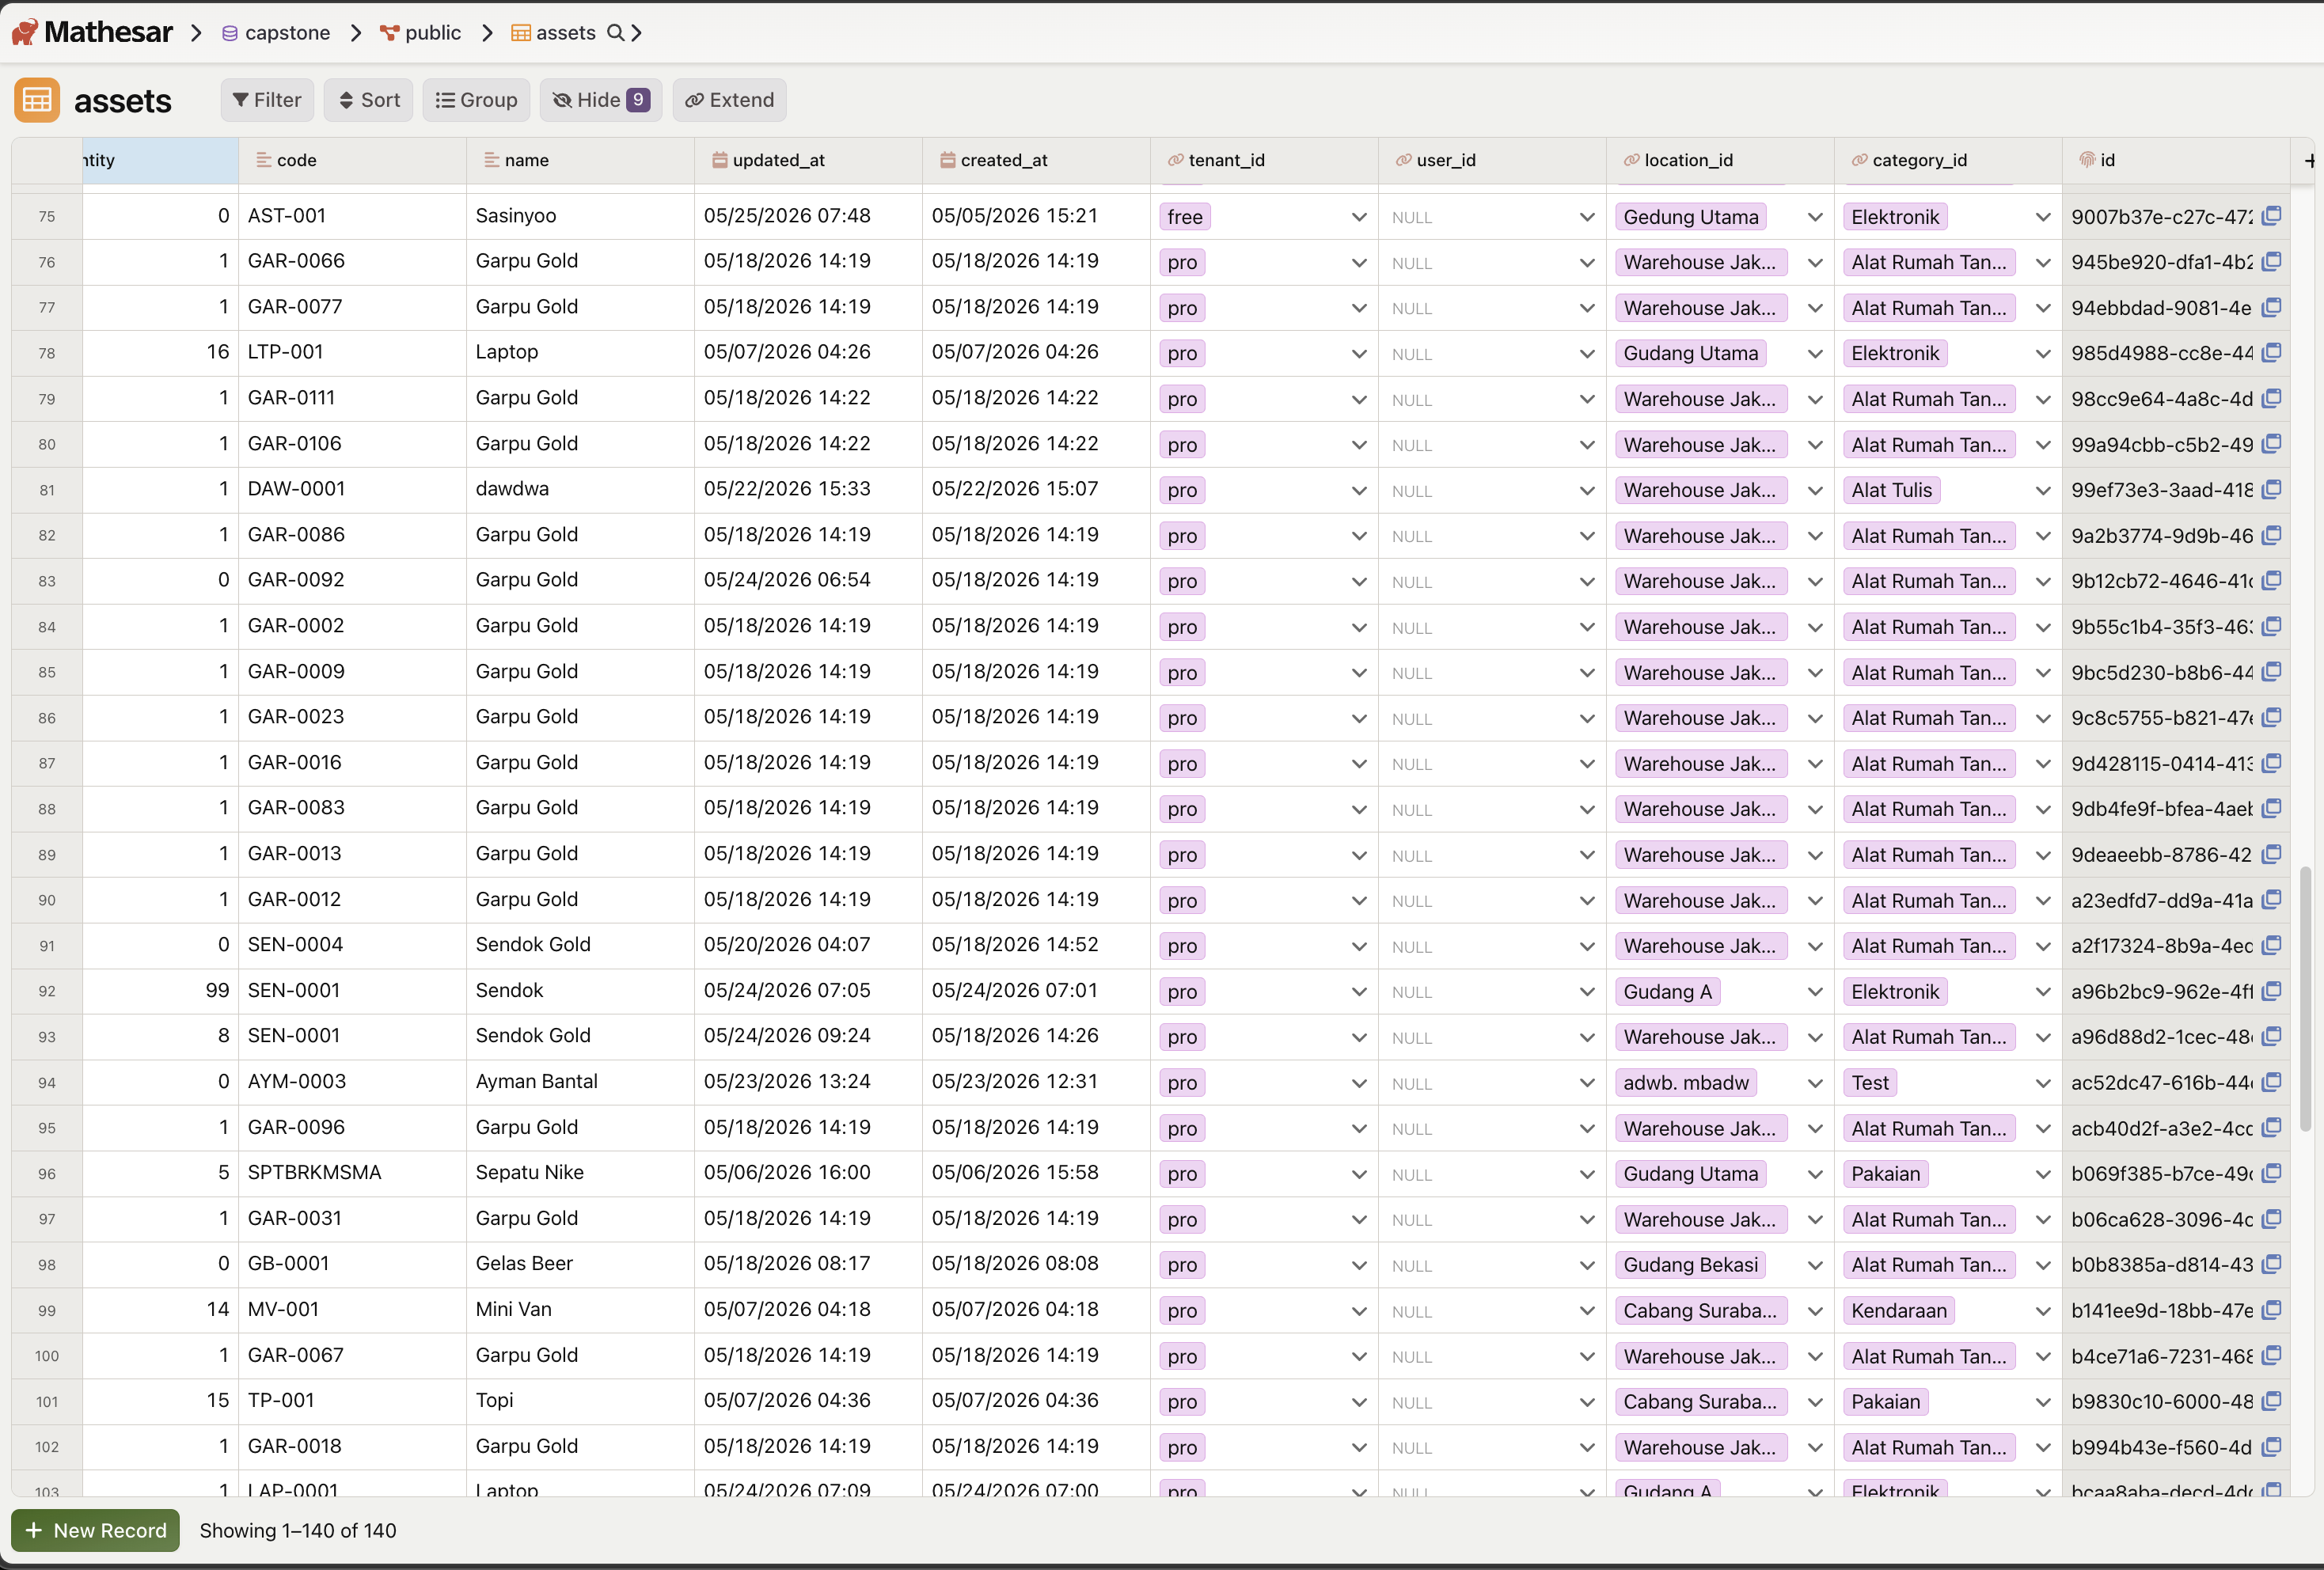
\includegraphics[width=0.9\textwidth]{assets/bab4/test3/table-asset.png}
  \caption{Data Multi \textit{Tenant} pada Tabel \textit{Assets}}
  \label{fig:data_multi_tenant_assets}
\end{figure}

Berdasarkan Gambar \ref{fig:data_multi_tenant_assets}, data aset dari beberapa \textit{tenant} tersimpan pada tabel \textit{assets} yang sama. Meskipun berada dalam satu tabel, setiap data memiliki atribut \textit{tenant\_id} yang berbeda. Atribut tersebut digunakan sebagai identitas \textit{tenant} sehingga sistem dapat membedakan kepemilikan data pada masing-masing \textit{tenant}.

Selain data aset, pengujian juga dilakukan terhadap data pengguna yang tersimpan pada sistem. Hasil pemeriksaan ditunjukkan pada Gambar \ref{fig:data_multi_tenant_users}.

\begin{figure}[H]
  \centering
  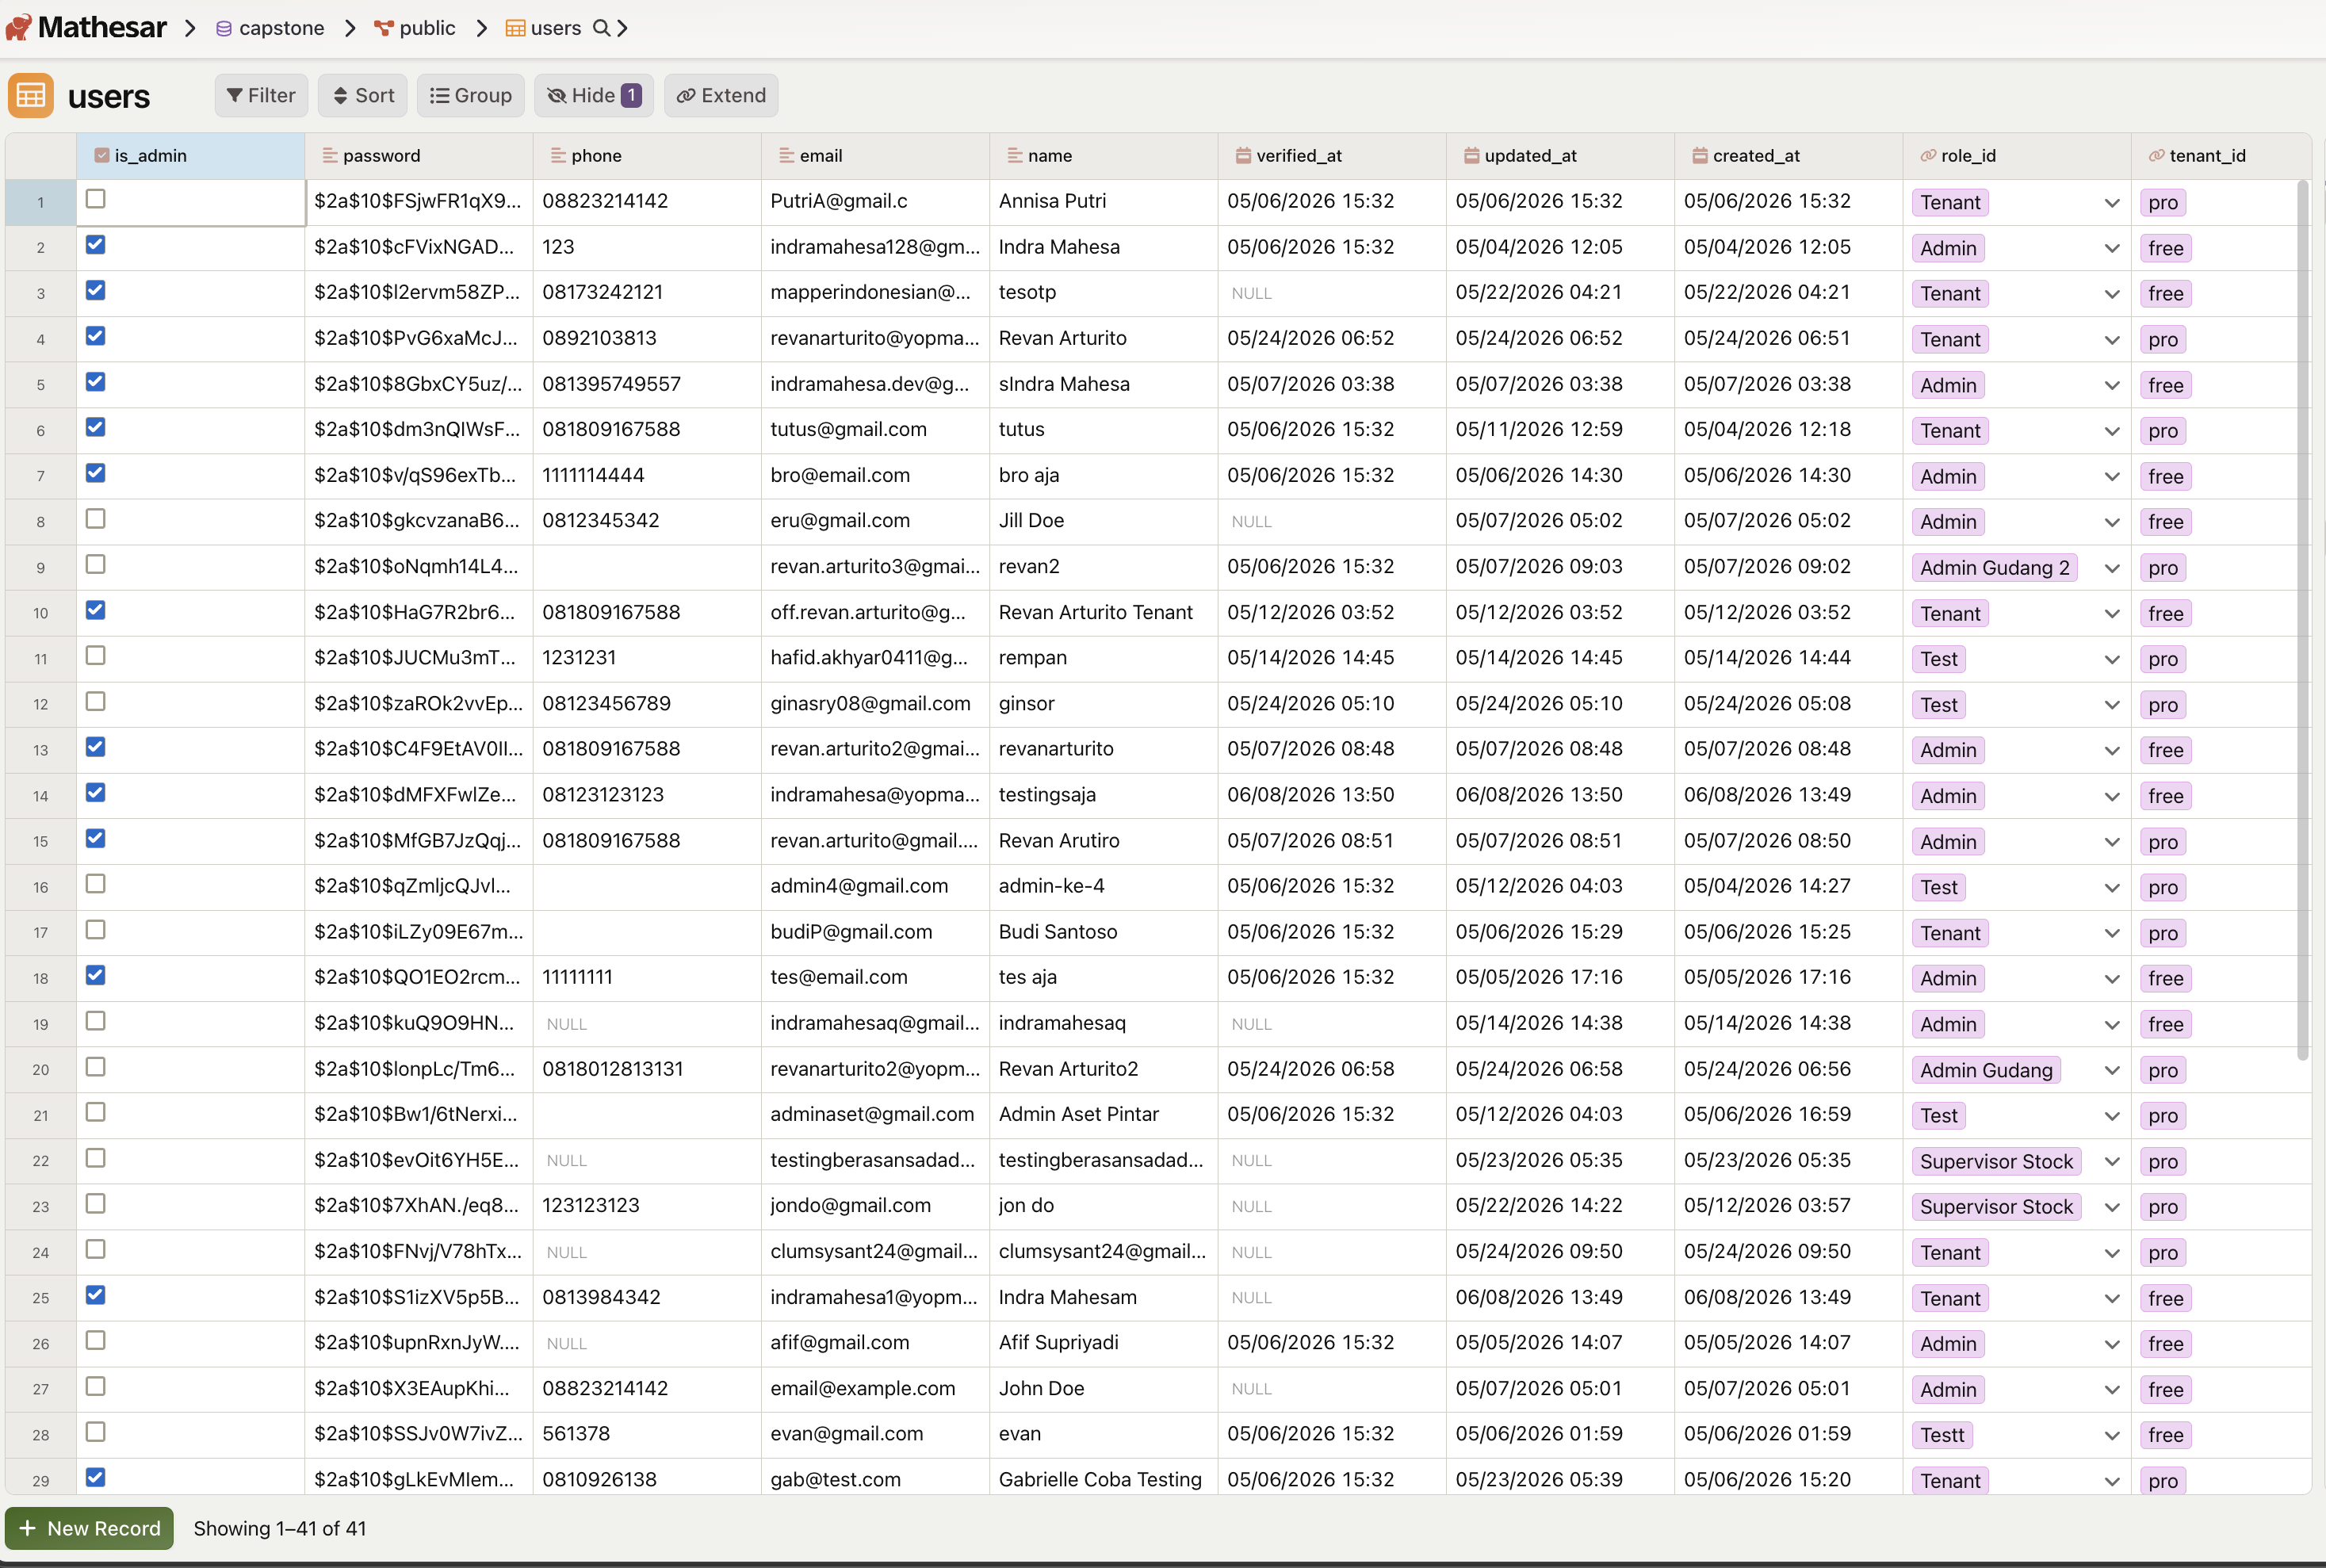
\includegraphics[width=0.9\textwidth]{assets/bab4/test3/table-user.png}
  \caption{Data Multi \textit{Tenant} pada Tabel \textit{Users}}
  \label{fig:data_multi_tenant_users}
\end{figure}

Berdasarkan Gambar \ref{fig:data_multi_tenant_users}, data pengguna dari beberapa \textit{tenant} juga tersimpan pada tabel \textit{users} yang sama. Setiap pengguna tetap memiliki keterkaitan dengan \textit{tenant} yang sesuai melalui atribut \textit{tenant\_id}. Hal tersebut menunjukkan bahwa pendekatan \textit{shared database} dan \textit{shared schema} diterapkan secara konsisten pada tabel yang digunakan oleh sistem.

Untuk memastikan bahwa \textit{tenant} menggunakan struktur tabel yang sama, dilakukan pemeriksaan terhadap skema tabel yang digunakan untuk menyimpan data operasional.

\begin{figure}[H]
  \centering
  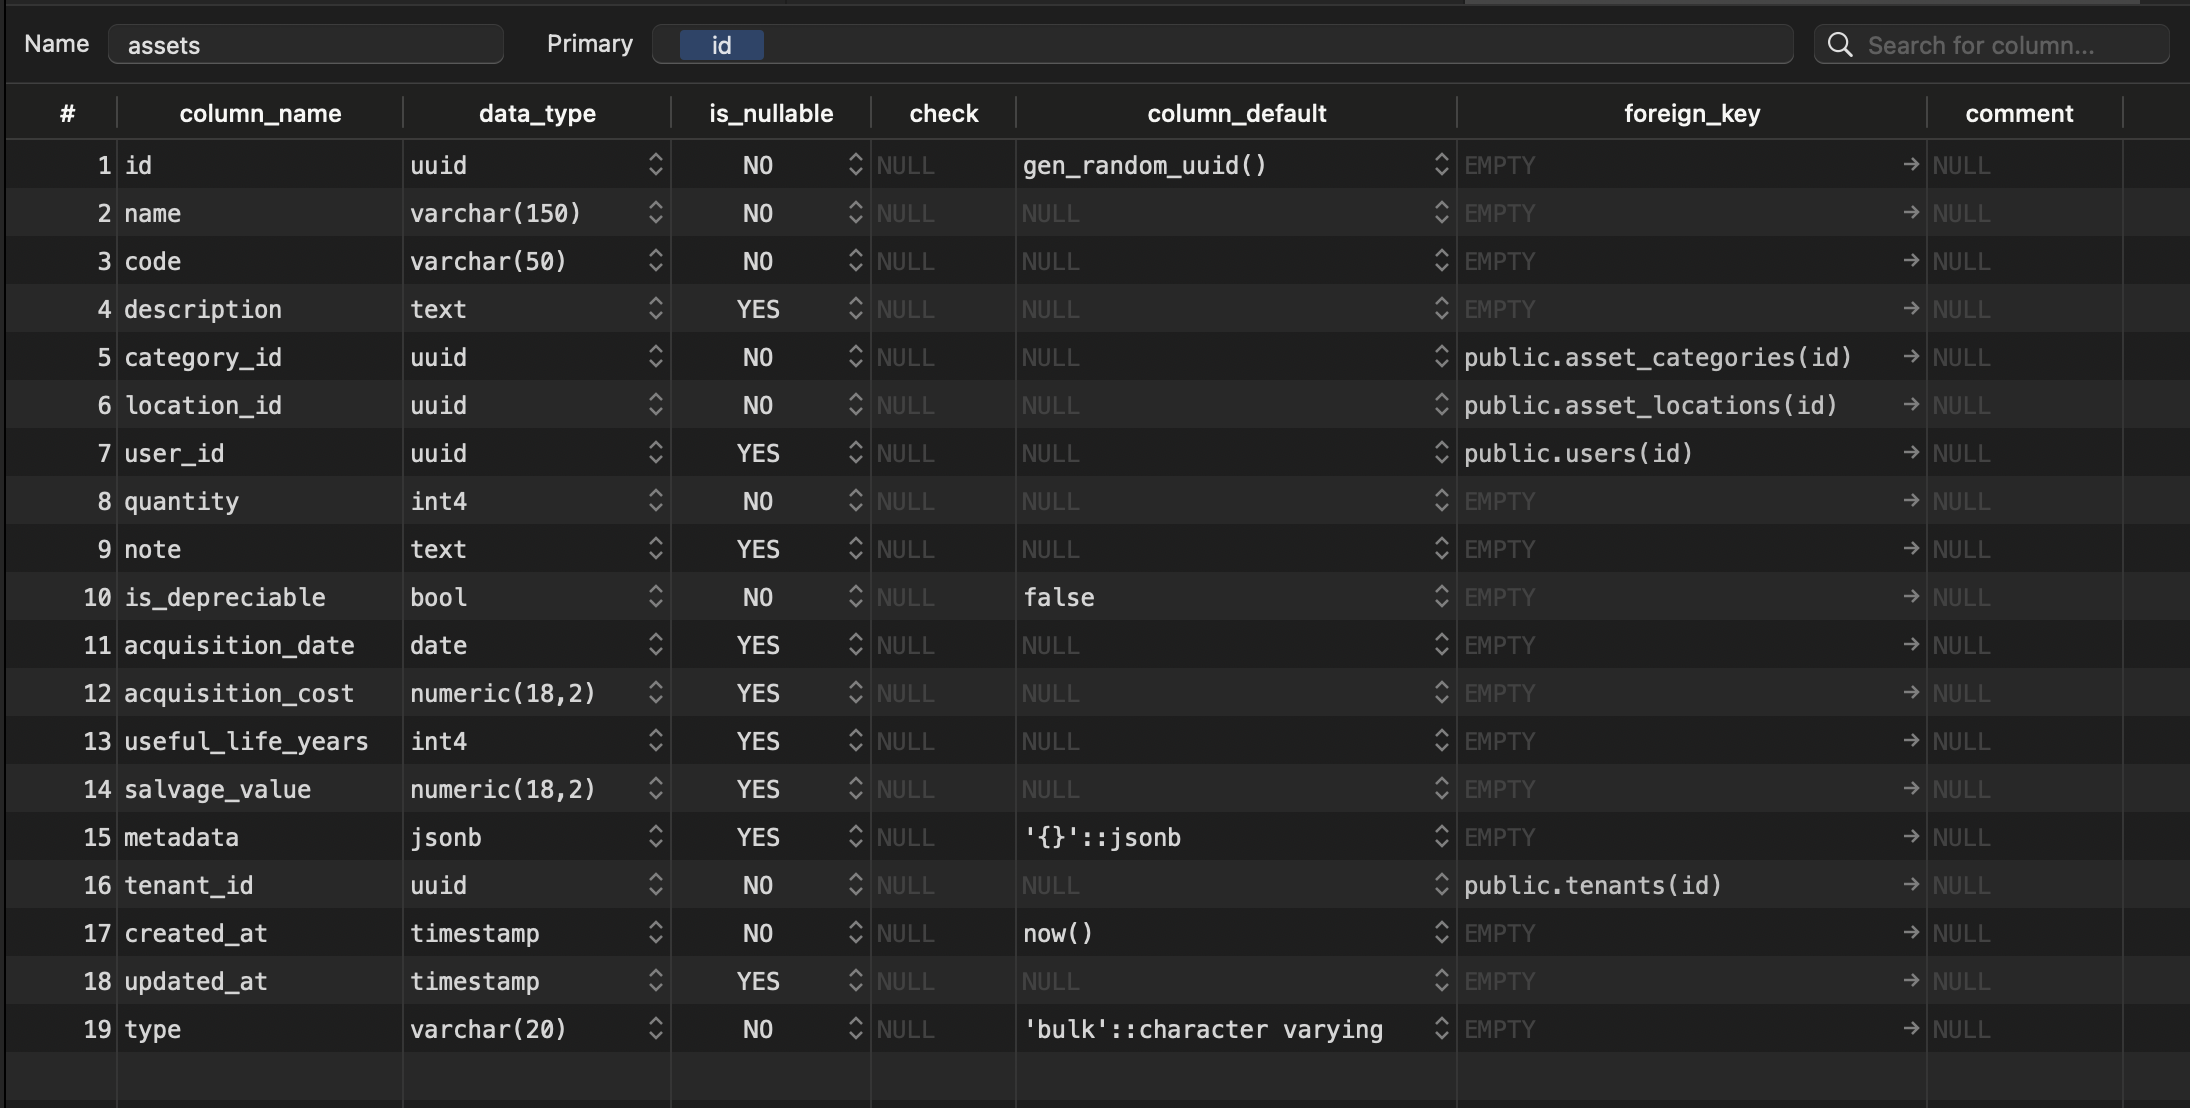
\includegraphics[width=0.9\textwidth]{assets/bab4/test3/structure-asset.png}
  \caption{Struktur Tabel \textit{Assets} pada Basis Data}
  \label{fig:struktur_tabel_assets}
\end{figure}

Gambar \ref{fig:struktur_tabel_assets} menunjukkan bahwa seluruh \textit{tenant} menggunakan struktur tabel yang sama untuk menyimpan data aset. Tidak terdapat tabel khusus untuk masing-masing \textit{tenant} sehingga seluruh data dikelola menggunakan satu skema basis data yang sama. Pendekatan ini memungkinkan pengelolaan basis data menjadi lebih sederhana dibandingkan penggunaan basis data atau tabel terpisah untuk setiap \textit{tenant}.

Hasil pengujian juga menunjukkan bahwa proses penyimpanan data dari \textit{tenant} yang berbeda dapat dilakukan tanpa menimbulkan konflik pada struktur basis data. Identifikasi \textit{tenant} dilakukan menggunakan atribut \textit{tenant\_id} yang disimpan pada setiap data operasional.

Ringkasan hasil pengujian \textit{shared database} dan \textit{shared schema} ditunjukkan pada Tabel \ref{tab:hasil_pengujian_shared_database}.

\begin{table}[H]
  \centering
  \caption{Hasil Pengujian \textit{Shared Database} dan \textit{Shared Schema}}
  \label{tab:hasil_pengujian_shared_database}
  \footnotesize
  \begin{tabular}{|l|>{\raggedright\arraybackslash}p{3.2cm}|>{\raggedright\arraybackslash}p{3.5cm}|>{\raggedright\arraybackslash}p{3.5cm}|>{\raggedright\arraybackslash}p{1.8cm}|}
    \hline
    \rowcolor[HTML]{EFEFEF}
    \textbf{No} & \textbf{Skenario Pengujian} & \textbf{Hasil yang Diharapkan} & \textbf{Hasil Aktual} & \textbf{Status} \\
    \hline
    1 & Tenant A menambahkan data aset & Data berhasil tersimpan pada tabel \textit{assets} & Data berhasil tersimpan pada tabel \textit{assets} & Berhasil \\
    \hline
    2 & Tenant B menambahkan data aset & Data berhasil tersimpan pada tabel \textit{assets} & Data berhasil tersimpan pada tabel \textit{assets} & Berhasil \\
    \hline
    3 & Pemeriksaan tabel \textit{assets} & Data beberapa \textit{tenant} berada pada tabel yang sama & Data beberapa \textit{tenant} berada pada tabel yang sama & Berhasil \\
    \hline
    4 & Pemeriksaan tabel \textit{users} & Data beberapa \textit{tenant} berada pada tabel yang sama & Data beberapa \textit{tenant} berada pada tabel yang sama & Berhasil \\
    \hline
    5 & Pemeriksaan atribut \textit{tenant\_id} & Setiap data memiliki identitas \textit{tenant} yang sesuai & Setiap data memiliki identitas \textit{tenant} yang sesuai & Berhasil \\
    \hline
    6 & Pemeriksaan struktur tabel & Seluruh \textit{tenant} menggunakan struktur tabel yang sama & Seluruh \textit{tenant} menggunakan struktur tabel yang sama & Berhasil \\
    \hline
  \end{tabular}
\end{table}

Berdasarkan hasil pengujian pada Tabel \ref{tab:hasil_pengujian_shared_database}, seluruh skenario pengujian berhasil dijalankan sesuai dengan hasil yang diharapkan. Data dari beberapa \textit{tenant} dapat disimpan pada tabel yang sama tanpa menyebabkan pencampuran data. Selain itu, setiap data tetap memiliki identitas \textit{tenant} yang dapat digunakan untuk membedakan kepemilikan data pada masing-masing \textit{tenant}.

Hasil tersebut menunjukkan bahwa implementasi \textit{shared database} dan \textit{shared schema} pada penelitian ini berhasil diterapkan sesuai dengan rancangan sistem. Pendekatan tersebut memungkinkan beberapa \textit{tenant} menggunakan basis data dan struktur tabel yang sama, namun tetap mendukung mekanisme pemisahan data melalui penggunaan atribut \textit{tenant\_id}.

\section{Analisis}

\subsection{Analisis Tenant Isolation}

Berdasarkan hasil pengujian yang telah dilakukan pada Subbab 4.3.1, mekanisme \textit{tenant isolation} berhasil diterapkan pada sistem sesuai dengan rancangan yang telah dijelaskan pada Bab 3. Hasil pengujian menunjukkan bahwa pengguna hanya dapat mengakses data yang berada dalam ruang lingkup \textit{tenant} yang sesuai dengan identitas \textit{tenant} yang dimiliki pengguna tersebut.

Pada pengujian menggunakan akun \textbf{gab@test.com} dan \textbf{indramahesa128@gmail.com}, sistem menampilkan data aset yang berbeda untuk masing-masing pengguna meskipun data tersebut tersimpan pada basis data dan tabel yang sama. Hasil tersebut menunjukkan bahwa sistem berhasil melakukan pemfilteran data berdasarkan identitas \textit{tenant} sebelum data dikembalikan kepada pengguna.

Selain melalui antarmuka aplikasi, hasil pengujian pada layanan API juga menunjukkan bahwa data yang dikembalikan sistem hanya berasal dari \textit{tenant} yang sedang aktif. Informasi \textit{tenant} yang tersimpan pada token autentikasi digunakan sebagai dasar untuk membatasi ruang lingkup akses data. Dengan mekanisme tersebut, pengguna tidak dapat memperoleh data milik \textit{tenant} lain meskipun menggunakan \textit{endpoint} API yang sama.

Berdasarkan indikator keberhasilan yang telah ditetapkan pada Bab 3, seluruh skenario pengujian \textit{tenant isolation} berhasil memenuhi kriteria yang diharapkan. Pengguna tidak dapat melihat, mengubah, maupun menghapus data yang dimiliki \textit{tenant} lain. Hasil tersebut menunjukkan bahwa mekanisme \textit{tenant isolation} yang diterapkan mampu menjaga pemisahan data antar \textit{tenant} secara konsisten pada lapisan aplikasi, layanan API, dan basis data.

\subsection{Analisis Tenant Provisioning}

Berdasarkan hasil pengujian pada Subbab 4.3.2, proses \textit{tenant provisioning} berhasil dijalankan sesuai dengan rancangan sistem yang telah dibuat. Seluruh tahapan yang dirancang, mulai dari registrasi \textit{tenant}, verifikasi email menggunakan kode OTP, hingga pembentukan data \textit{tenant} dan akun administrator, berhasil dilakukan secara otomatis oleh sistem.

Hasil pengujian menunjukkan bahwa setelah pengguna menyelesaikan proses registrasi dan verifikasi email, sistem secara otomatis membentuk data \textit{tenant}, \textit{role} administrator, relasi \textit{permission}, dan akun administrator tanpa memerlukan konfigurasi manual tambahan. Pendekatan tersebut memungkinkan \textit{tenant} yang baru terdaftar dapat langsung menggunakan sistem setelah proses registrasi selesai dilakukan.

Selain meningkatkan efisiensi proses \textit{onboarding} \textit{tenant}, mekanisme \textit{tenant provisioning} juga membantu menjaga konsistensi konfigurasi pada setiap \textit{tenant} yang terdaftar. Seluruh \textit{tenant} memperoleh struktur \textit{role} dan hak akses awal yang seragam sehingga risiko kesalahan konfigurasi dapat diminimalkan.

Berdasarkan indikator keberhasilan yang telah ditetapkan pada Bab 3, seluruh kasus uji pada proses \textit{tenant provisioning} berhasil memenuhi hasil yang diharapkan. Dengan demikian, mekanisme yang diterapkan pada penelitian ini mampu mendukung proses pendaftaran \textit{tenant} baru secara otomatis dan mempersingkat proses aktivasi \textit{tenant} pada sistem \textit{multitenant}.

\subsection{Analisis Shared Database dan Shared Schema}

Berdasarkan hasil pengujian pada Subbab 4.3.3, implementasi \textit{shared database} dan \textit{shared schema} berhasil diterapkan sesuai dengan rancangan yang diusulkan. Hasil pemeriksaan basis data menunjukkan bahwa data dari beberapa \textit{tenant} dapat disimpan pada basis data dan struktur tabel yang sama tanpa menyebabkan pencampuran data antar \textit{tenant}.

Penggunaan atribut \textit{tenant\_id} pada setiap data operasional memungkinkan sistem mengidentifikasi kepemilikan data dari masing-masing \textit{tenant}. Meskipun data aset dan pengguna berada pada tabel yang sama, setiap data tetap dapat dibedakan berdasarkan identitas \textit{tenant} yang dimiliki. Hasil tersebut menunjukkan bahwa pendekatan \textit{shared database} dan \textit{shared schema} dapat digunakan tanpa mengurangi kemampuan sistem dalam menjaga pemisahan data.

Penerapan pendekatan ini juga memberikan keuntungan dalam pengelolaan basis data karena seluruh \textit{tenant} menggunakan struktur tabel yang sama. Dengan demikian, proses pengembangan dan pemeliharaan basis data dapat dilakukan secara lebih sederhana dibandingkan pendekatan yang menggunakan basis data atau tabel terpisah untuk setiap \textit{tenant}.

Berdasarkan indikator keberhasilan yang telah ditetapkan pada Bab 3, seluruh skenario pengujian berhasil memenuhi kriteria yang diharapkan. Data dari beberapa \textit{tenant} berhasil disimpan pada tabel yang sama dan tetap dapat dipisahkan melalui atribut \textit{tenant\_id}. Hasil tersebut menunjukkan bahwa implementasi \textit{shared database} dan \textit{shared schema} yang digunakan pada penelitian ini berhasil mendukung kebutuhan arsitektur \textit{multitenant} yang diterapkan pada sistem.
